\documentclass[12p,a4paper]{report} 	
\usepackage{pslatex}
\usepackage[nottoc,notlot,notlof]{tocbibind}
\usepackage{tocloft}

\renewcommand\cftchapafterpnum{\vskip5pt}
\renewcommand\cftsecafterpnum{\vskip0pt}
\renewcommand\cftsubsecafterpnum{\vskip0pt}
\usepackage{tikz}
\usetikzlibrary{arrows}
\usepackage[utf8]{inputenc}
\usepackage{sectsty}
\usepackage[titletoc]{appendix}
\usepackage{url}
\usepackage{listings}
\usepackage{graphicx}
\usepackage{float}
\usepackage{wrapfig}
\usepackage{amsmath}
\usepackage{natbib}

\usepackage{indentfirst}
\usepackage{listingsutf8}
\setlength{\parskip}{2ex}

\title{}
\author{}

\renewcommand{\bibname}{References}
\setcounter{tocdepth}{4}
\setcounter{secnumdepth}{4}
\usepackage{color}
\begin{document}

\begin{center}
\Large COMP30040 Project Report \\ \vspace{10pt} \huge Wirelessly Controlled Robot Through  \\ Advanced Arm Motion Capture, Tracking and Gesture Recognition
\end{center}

\vspace{30pt}
\begin{center} \Large  \emph{Submitted in partial fulfillment of the requirements for the award of the degree of} \\ \vspace{10pt}

\textbf{\large BSc(Hons) in Computer Science}

\Large By \\ \vspace{5pt}
\textbf{Radu Chichi} \\ \vspace{5pt} under the supervision of \\ \vspace{5pt}
\textbf{Dr. Paul Nutter}
\end{center}

\vspace{150pt}
	
\begin{center} \Large
School of Computer Science, Faculty of Engineering and Physical Sciences, The University of Manchester \\ April 2015 
\end{center}

	\newpage
\vspace*{130pt}
\begin{center}
\Large Abstract
\end{center}

This project explored the idea of building and controlling a robot composed of several subsystems, through the capture, tracking and recognition of arm and hand movements, achieved both optically, as well as through accelerometer and gyroscope readings. \\

This report is structured such that it provides an introduction as well as some background information regarding the topic of robotics and the various sensor technologies used. We will explain some of the goals and motivations, and finally look over the hardware and software solutions which have been explored and tested, as well as the mechanical engineering involved in building some of the structures required. Finally, we will showcase the end result, and present a short summary.

\newpage


\vspace*{150pt}
\begin{center} \Large Acknowledgements

\end{center}

\vspace{15pt}

I would like to thank my supervisor, \textbf{Dr. Paul Nutter}, for providing great guidance throughout the course of my final year, \textbf{my family }for the emotional support needed to overcome the stress that the final year of university comes to bear, \textbf{my team} at \textbf{Microsoft} for being understanding and not giving me a lot
of work to do during my part-time role whilst studying, and, perhaps most importantly, I would like to thank \textbf{Steve Rhodes}, for the invaluable help offered throughout the course of this project. Without Steve, this project would not have progressed to this stage. \\

Finally, I would also like to thank the \textbf{School of Computer Science} at \textbf{The University of Manchester} for providing me with an invaluable education, as well as access to all the resources required for fostering my development. Thanks!

\newpage

\tableofcontents

\newpage

\listoffigures
\newpage
\sectionfont{\huge}
\subsectionfont{\LARGE}
\partfont{\Large}

\chapter{Introduction}
This chapter will provide some background information regarding the field of \textbf{robotics}, explaining the notion as well as providing some insight into the main drivers/goals of the field. It will also provide a brief introduction to the field of \textbf{Human-Computer Interaction (HCI)}. Finally, it will outline some of the initial goals of the project.

\section{Background Information}
\subsection{Robotics}
The field of \textbf{robotics} unites several areas of study, ranging from mechanical engineering, electrical engineering, electronics and computer science, in order to create autonomous or remote controlled assemblies. These so called assemblies are referred to as \textbf{robots}, a term originating from the Slavic word \textbf{robota}, meaning labor \cite{robota}. Their usage varies, being used in order to speed up existing processes and reduce the amount of menial tasks human laborers would have to carry out, or to provide functionality which would otherwise be either unattainable or that could pose a significant threat to a human being. \\

Given the wide applicability and possible configurations a robot can have, their design is fundamentally based on the goal they need to accomplish. Upon design, factors to take into consideration include:
\begin{itemize}
\setlength\itemsep{-0.2em}
\item \textbf{Body} - The body of a robot can vary widely, being highly dependent on its specific purpose.
\item \textbf{Power System} - The power system is responsible for providing, most oftenly, a supply of \textbf{direct current (DC)} to all the robot's subsystems. For non-mobile robots, usage of \textbf{AC adaptors} is standard. Mobile robots will require either batteries, or another source of energy. For complex systems, it is common to see a centralized supply, with voltage regulators for each of the robot's subsystems. 
\item \textbf{Locomotion} - For mobile robots, the locomotion system forms a crucial part of their design. There are numerous aspects to take into consideration when designing a moving assembly, aspects which will be covered further down.
\item \textbf{Manipulation} - Done in order to avoid exposing humans to direct contact, or to automate certain tasks.
\item \textbf{Programming} - The software that will govern the robot's behavior is a fundamental component. The software can be classified as having three main variations:
\begin{itemize}
\item \textbf{Fully Autonomous} \\
	In the instance of fully independent robots, the behavior of the robot has to either be programmed, such that it follows a predefined set of instructions, or, alternatively, have it be programmed in such a way that it can learn and adapt on its own. Most industrial, commercial and military robots perform simple, repetitive tasks.
	\item \textbf{Remote Controlled} \\
	Remote Controlled robots are controlled from a distance by a human operator. This report will be centered on developing such a robot.
	\item \textbf{Semi-autonomous} \\
	Semi-autonomous robots retain characteristics of both fully autonomous, as well as remotely controlled robots.
\end{itemize}

\end{itemize}


\subsection{Human-Computer Interaction}
Another crucial area in the field of robotics is that of \textbf{Human-Computer Interaction}. This is more evident in the case of remotely operated robots, and it will be the main focus of our investigation. \\

The basic goal of the field is to construct more natural interfaces between humans and computers. Most of the current research aims to create interfaces driven solely by speech or voice, making control more natural, and eliminating the need for the user to operate any specific input device.

\section{Project Goals and Motivation}
The initial goal of the project was to interface an off the shelf robotic arm with a device capable of tracking arm movements, such as the \textbf{Microsoft Kinect}, or the \textbf{Leap Motion}. The project goals have been revisited throughout the development period, and expanded to that of creating a gesture-based wirelessly controlled robot, consisting of a robotic arm with locomotive capabilities.

\chapter{Background and Research}
This chapter will expand upon the brief background presented in \textbf{Chapter I}, touching upon each of the components that will form the final project. These components can be distilled into:
\begin{itemize}
\item \textbf{Motion Capture} - Needed in order to determine the user's commands and the actions the robot needs to perform.
\item \textbf{Robotic Assembly} - Consisting of all the subsystems which will be controlled remotely.
\item \textbf{Telecommunication} - Needed in order to relay the data captured by \textbf{Motion Capture} to the \textbf{Robotic Assembly}, as well as relaying telemetry back to the user in order to inform the user of the robot's surroundings and current configuration.  
\end{itemize}

\section{Motion Capture} 
\textbf{Motion Capture} (abbreviated \textbf{Mo-cap}) is a process used to infer the movements of people, objects or animals. The field saw its first development in the medical field, being used for biomechanics research as a photogrammetric analysis tool to study human motion \cite{mocap}. Since then, the field has expanded, becoming popular in animation, easing the animation process through the use of human actors. It also has applicability in military, entertainment, virtual reality, sports, medical applications, and for validation of computer vision and robotics \cite{mocapapp}. \\

In the last few years, usage has become even more widespread, given the introduction of such technologies to the consumer market. Notable mentions include the \textbf{Microsoft Kinect}, \textbf{Leap Motion}, \textbf{PrimeSense Carmine}, etc.

Throughout this section, we will investigate several methods which can be used for tracking the human movements in 3D space.

\newpage
\subsection{Optical Systems}
Optical systems use light in order to determine the user's pose. These fall into two large, and mostly distinct categories.
\begin{itemize}
\item \textbf{Marker based Tracking} - In this technique, reflective markers are placed on the human body. By using several cameras, a three dimensional fix can be acquired. A slightly varied technique is to use \emph{active} markers, whereby LED markers are placed on the user instead.

\item \textbf{Markerless Tracking} - This technique permits tracking without use of any markers, by using computer vision and machine learning algorithms in order to extrapolate a pose from a given image. In the case of the \textbf{Microsoft Kinect}, tracking is accomplished through a two-way process (Figure \ref{fig:microsoftkinectbody}):

\begin{figure}[H]
\begin{center}

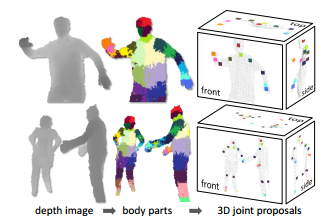
\includegraphics{kinectbodyparts}
\caption{Outline of the mapping process. \cite{microsoftkinectbody}}
\label{fig:microsoftkinectbody}
\end{center}
\end{figure}
				
	\begin{itemize}
		\item Acquiring a \textbf{depth map} of the scene. A depth map is defined as being an image, alongside information describing distances to all the surfaces within the image. The Kinect achieves this by emitting a \emph{known} pattern of infrared light (structured light). The scene's geometry will affect the way the pattern gets deformed, information which can be used to infer the distances to all the surfaces within the image \cite{microsoftkinectdepth}. 
		\item Once a depth map is acquired, the next step involves a per-pixel classification process which will assign it to one of several possible body parts \cite{microsoftkinectbody}. 
	\end{itemize}
\end{itemize}

\newpage

\subsection{Non-optical systems}
Non-optical systems require the user to wear equipment aimed to track joint movement. These mostly comprise of:

\begin{itemize}
\item \textbf{Inertial Systems} - Requires the user to wear a number of inertial sensors on their body. The data from all the sensors is then combined using various algorithms to create a model representing the user's pose.
\item \textbf{Mechanical Motion} - Requires the user to wear an exoskeleton that registers his moves by mechanically driving a set of gears.
\end{itemize}


\section{Robotic Assembly}

This section will cover several aspects of robotics that will form an integral part of the project.


\subsection{Robot Locomotion}

Robot locomotion is an important aspect to consider when designing mobile robots, as the type of locomotion will depend on the required use case. For the scope of this project, only terrestrial methods of locomotion will be investigated.

From a hardware aspect, the two main notions to consider when it comes to locomotion are:

\begin{itemize}
\item \textbf{Actuator Type} - The actuator is a type of motor used for controlling a mechanical system. These convert energy, such as electric current or hydraulic pressure into movement. A common example is the \textbf{DC motor}.
\item \textbf{Method used for Locomotion} - Robots might employ various methods for movement, most commonly using wheel based locomotion due to their simple nature and high effectiveness on flat surfaces. Other methods such as hopping or walking using artificial legs exist as well.
\end{itemize}

For the scope of the project and this report, only wheeled based locomotion achieved through \textbf{DC motors} will be explored in more depth.

A DC Motor is composed of two parts, a stator and a rotor. When subjected to a current, the rotor will spin, with the direction of rotation being a result of the polarity of the current, and the speed being governed by the voltage.

The speed can thus be controlled by varying the voltage of the source. A common technique in electronics is to use \textbf{Pulse Width Modulation (PWM)}, in order to vary the voltage. This technique is used to modulate a digital signal, in order to obtain an analog output. The modulation works by defining a regular interval of time, known as a \textbf{full cycle}, and the amount of time the signal is high within the full cycle, known as the \textbf{duty cycle}. The duty cycle is expressed as a percentage of the full cycle. In motor control, the percentage will correspond to the amount of voltage the motor will be subjected to (see \textbf{Figure \ref{fig:duty_cycle})}.

\begin{figure}[H]
\begin{center}
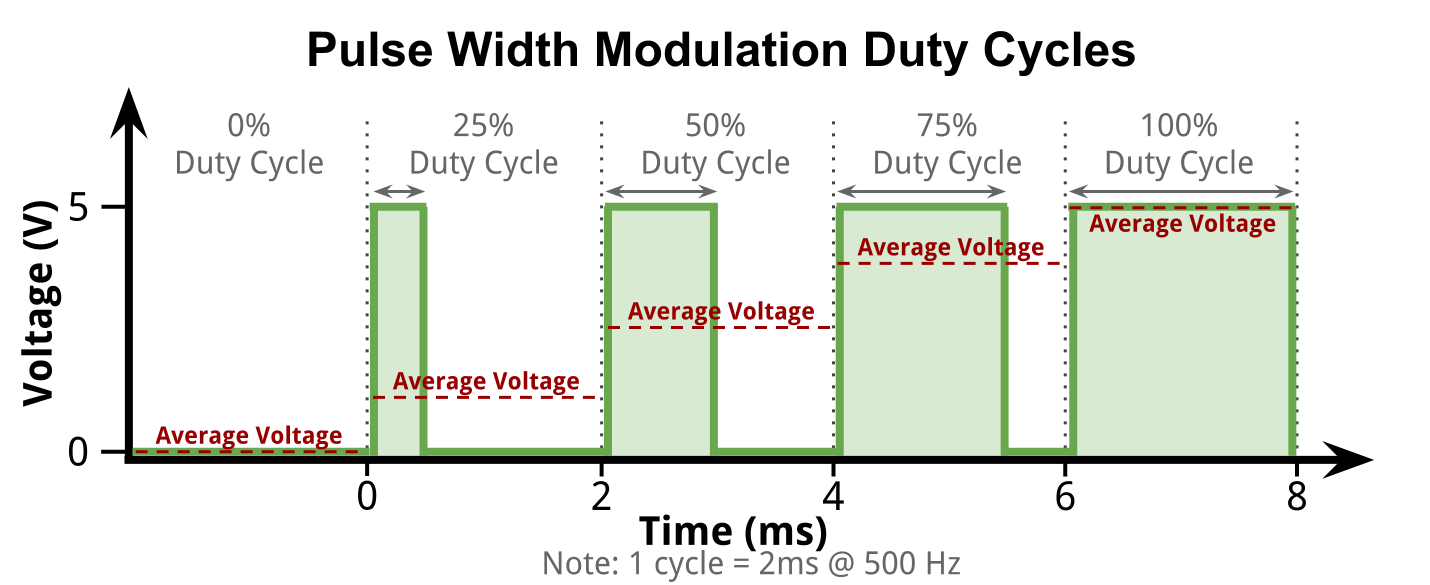
\includegraphics[scale=0.2]{duty_cycle}
\caption{PWM Outline \cite{duty_cycle}}
\label{fig:duty_cycle}
\end{center}
\end{figure}

\subsubsection{Steering}

In order for a mobile robot to move freely, it requires steering capability. Conventional wheel-based steering is not necessarily ideal, due to the multitude of components required in order to be able to pivot the wheels.

Differential steering has seen wide usage in robotics, mostly due to ease of implementation, as well as the ability to rotate in place \cite{diffsteering}. By having the set of wheels on each side rotate independently of each other, the assembly is able to steer. In-place steering can be achieved by steering one side in the opposite direction to the other.

\begin{figure}[H]
\begin{center}
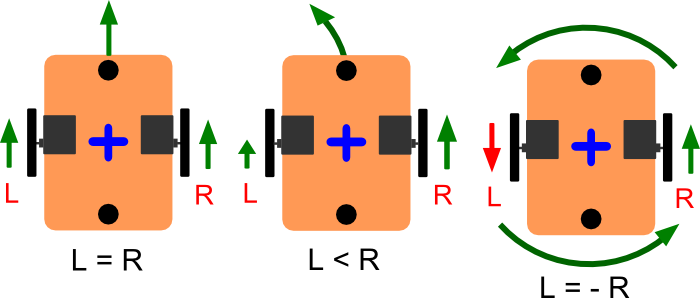
\includegraphics[scale=0.6]{differential-steering}
\caption{Outline of differential steering. \textbf{L} represents the speed of the track on the left side, whilst \textbf{R} represents the speed on the right side. \cite{differential-steering}} 
\label{fig:differential-steering}
\end{center}
\end{figure}
\newpage

\subsection{Robot Manipulation}

In various scenarios, robots are required to manipulate objects. Depending on the use case, they may be required to pick up, position, weld etc.

To this end, a robotic arm of some description is required. A robotic arm is a mechanical assembly that mimics a human arm, consisting of several joints operated by a series of actuators which control the movements. The links within the arm form a so called kinematic chain, whereby the configuration of a joint will affect the position of any subsequent part. The end of the arm is known as an \textbf{'end-effector'}, its exact specification varying in accordance to the requirements \cite{endeffector}. The movements of the actuators are controlled by a microcontroller, usually located at the base of the arm. An arm, as such, can be programmed to execute a variety tasks, which can vary from use case to use case.

The actuators that operate the arm need to provide enough torque in order to hold both the weight held by the end-effector, if any, as well as support the arm's own weight.

Additionally, the actuators have to provide precise positioning, and maintain their required position under load. \textbf{Servomotors} can be used to this end, allowing for precise control of position and speed, by employing a feedback mechanism.  

\begin{figure}[H]
\begin{center}
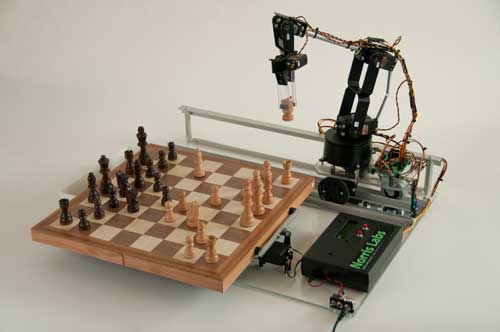
\includegraphics[scale=0.7]{ChessBot}
\caption{An example of a robotic arm picking up chess pieces. \cite{chessbot}}
\label{fig:ChessBot}
\end{center}
\end{figure}


\newpage

\begin{figure}
\begin{center}

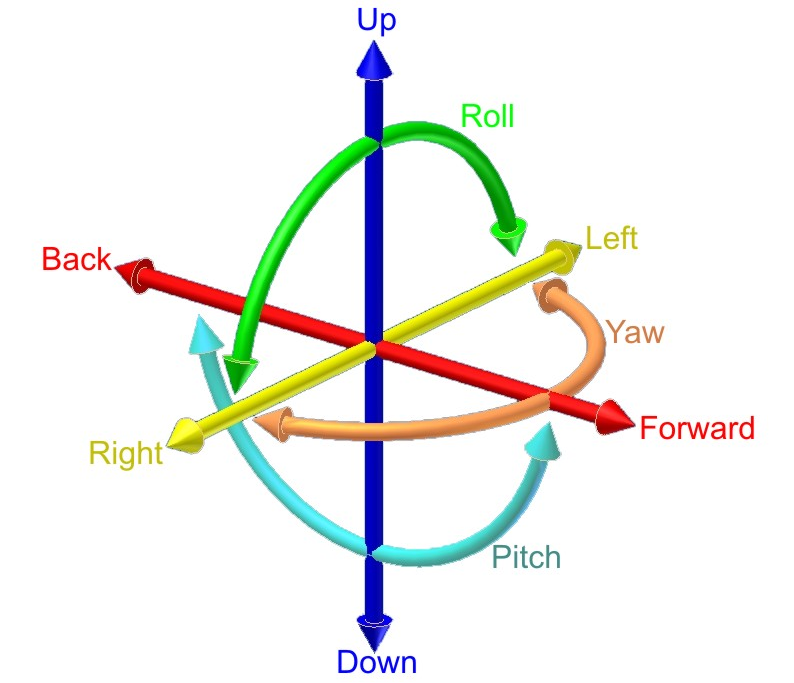
\includegraphics[scale=0.40]{6DOF_en}
\caption{6 degrees of freedom \cite{6dof}}
\label{fig:6dof}
\end{center}
\end{figure}

It can be seen that in 3-dimensional space, any possible position and orientation can be described through the use of  \textbf{6 parameters}, 3 corresponding to a position in space (commonly denoted \textbf{x, y, z}), and 3 corresponding to orientations in all of the three dimensions, referred to as \textbf{roll, pitch and yaw}. (denoted in \textbf{Figure \ref{fig:6dof}}). The number of parameters needed to describe the configuration of a mechanical system is considered to be the number of \textbf{degrees of freedom (DoF)} the system has.\\

\section{Telecommunication}
In order for a robot to be controlled from a distance, user commands have to be passed to the robot. In addition, information regarding the robot's environment has to be passed back to the controller. There are numerous networking models one could consider when designing such a system. Control through the \textbf{Internet Protocol suite} could provide virtually unlimited range, if connected through the Internet using Wi-Fi. Other models which could prove more suitable for short distance communication include Bluetooth and RF, amongst others.

The sensor data that gets sent back to the controller will be specific to the use case. Among many others, ones to note include visual feed, audio feed, accelerometer/gyroscope data, GPS data, etc.


\chapter{Hardware Design}

This chapter will describe a design of the whole system, including the different technologies which will be needed.
Due to the nature of the components used, two \textbf{independent} control systems will be required.
 
\section{Robot Body}
The body will be the main structure of the robot, being required to house all the various subsystems. Due to the size and number of the various components, a considerably sized structure will be required. An \textbf{inverse T shaped} structure was devised, providing a tall and flat surface area for attaching the arm, as well as having a base with a large surface area, providing increased stability. 

The final structure has been made out of wood, due to both being easy to process, as well as being readily available (See \textbf{Figure \ref{fig:robot_body2}}). The structure has considerable weight, providing additional stability, due to inertia.

\begin{figure}[H]
\begin{center}
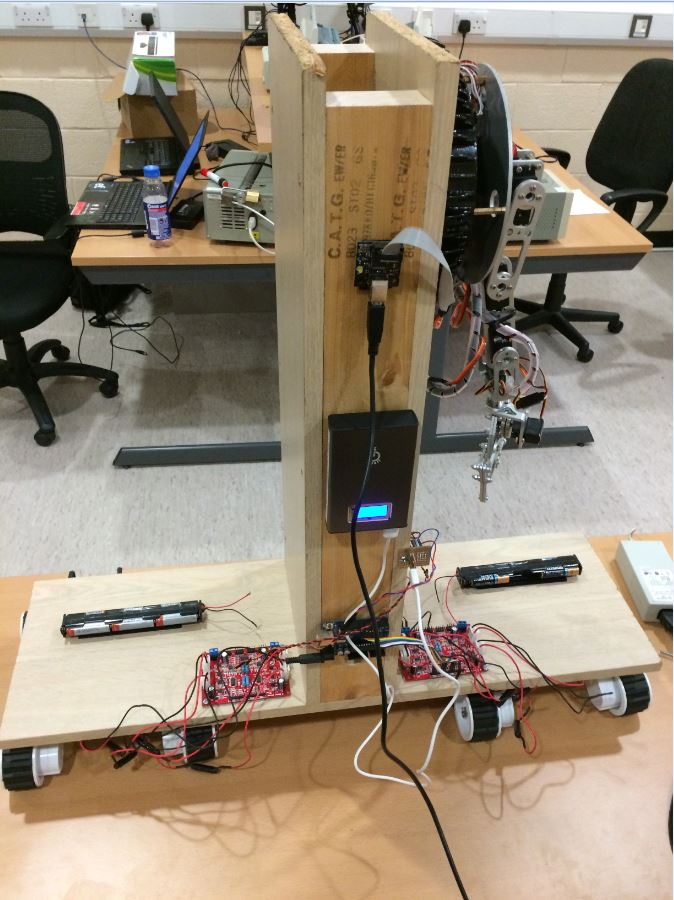
\includegraphics[scale=0.50]{robot_body_low}
\caption{Photo of the Robot taken in early development. Other components that are visible in the photo will be discussed further down.}
\label{fig:robot_body2}
\end{center}
\end{figure}


\section{Robotic Arm Assembly}


The \textbf{Robotic Arm Assembly} will consist of all the hardware and software components that will allow the user to drive a robotic arm. A wireless interface between the \textbf{robot arm and a computer} will be devised in order to allow remote operation through natural movements. Several sensors and output devices will be connected to the main computer, which will relay the necessary data to the robotic arm.
\newpage

\subsection{Robot Arm}

\begin{wrapfigure}{r}{0.5\textwidth}
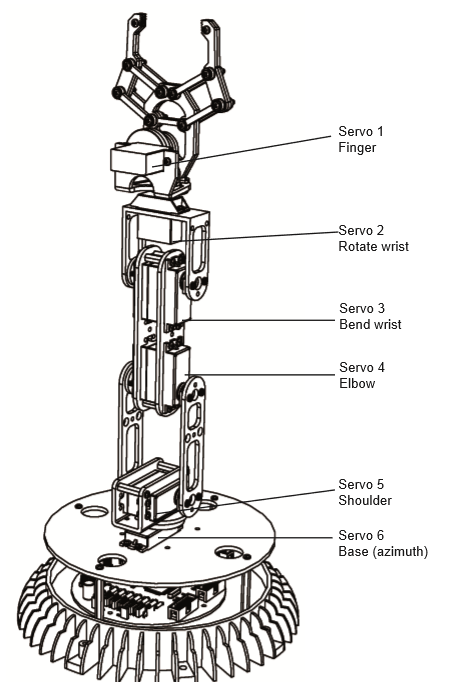
\includegraphics[scale=0.65]{robotarm}
\caption{RA1-Pro Robotic Arm \cite{arexx}}
\label{fig:robotarm}
\end{wrapfigure}

The Robotic Arm that will be operated is the \textbf{AREXX RA1-Pro}, an off-the shelf robotic arm. The arm, as depicted  in \textbf{Figure \ref{fig:robotarm}}, is operated by \textbf{6 servomotors}, 5 operating the joints, providing translation and rotation capabilities, and one motor operating the gripper. This provides the arm with \textbf{5 degrees of freedom (DoF)}. It is important to understand that the space representing the number of possible positions the arm can achieve is directly correlated to its \textbf{DoF} number. Thus, any possible configuration can be described by providing 5 parameters, corresponding to the 5 actuators.

The \textbf{RA1-Pro} will be operated remotely, through the \textbf{APC220 Radio Communication Module}. The module has been chosen since it provides a low powered, easy to integrate solution, being able to operate at considerable ranges (of up to 1000m) \cite{apc220range}. The full communication assembly will consist of two APC220 modules, one connected directly to the RA1-PRO PCB (please refer to \textbf{Appendix A}), and one connected to a laptop which will provide control, connected via \textbf{USB} through a \textbf{UART/TTL adapter}. 

Communication to the arm is done through a \textbf{Serial Universal Asynchronous Receiver/Transmitter using Transistor-transistor Logic} (\textbf{UART/TTL} for short) interface.  It is labeled universal since it does not use a clock in order to synchronize communication between devices. As such, the rate of communication (known as baud rate), needs to be agreed beforehand by both parties. 

\newpage
On each end, when a UART module receives a word of information to send, it adds a start bit and end bit to the beginning and end of the word, and optionally a parity bit to provide error correction capabilities. It then proceeds to send the data in a sequential fashion, according to a preset baud rate. Once the receiver intercepts the first bit (given by a voltage transition), it can infer, given the baud rate, when the next transition will occur. Note that the UART has an internal clock which operates at a multiple of the data rate \cite{uart} (Refer to \textbf{Figure \ref{fig:uart}}).

\begin{figure}[H]
\begin{center}
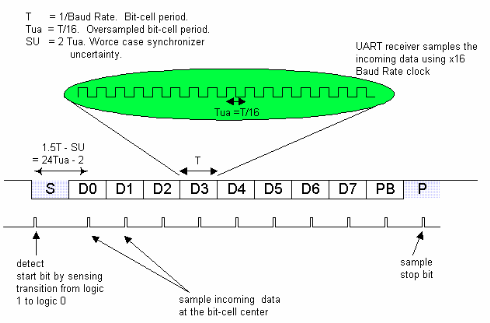
\includegraphics{uartreceiver}
\caption{UART Receiver depicted receiving a word of data by several impulses at fixed intervals apart, represented from voltage transitions.\cite{uart}}
\label{fig:uart}
\end{center}
\end{figure}

\textbf{TTL} refers to a hardware description of the UART protocol. It operates on only two \textbf{digital} lines (known as \textbf{RX} and\textbf{TX}), one of them being used for sending, while the other one is being used for reading incoming data (See \textbf{Figure \ref{fig:uart}}). The protocol as such can be considered to be full duplex, since it allows both devices to communicate to each other. 

The TTL standard defines a \emph{high} signal being represented by a voltage of \textbf{5V}, and a \emph{low} signal being given by a lack of any voltage.

\begin{figure}[H]
\begin{center}
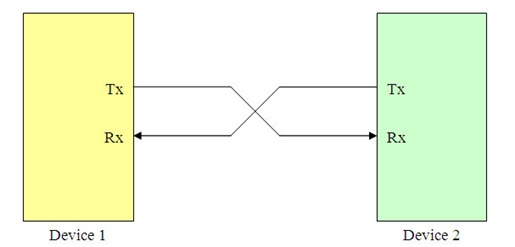
\includegraphics[scale=0.40]{uart}
\caption{TTL Depiction \cite{uart}}
\label{fig:uart}
\end{center}
\end{figure}
\newpage
Thus, the joint parameters will be computed on a computer, remotely, and relayed to the arm using the \textbf{UART/TTL} interface described previously (denoted in \textbf{Figure \ref{fig:ttlinterface}}). The parameters will then be used to drive the actuators on the arm.

\begin{figure}[H]
\begin{center}
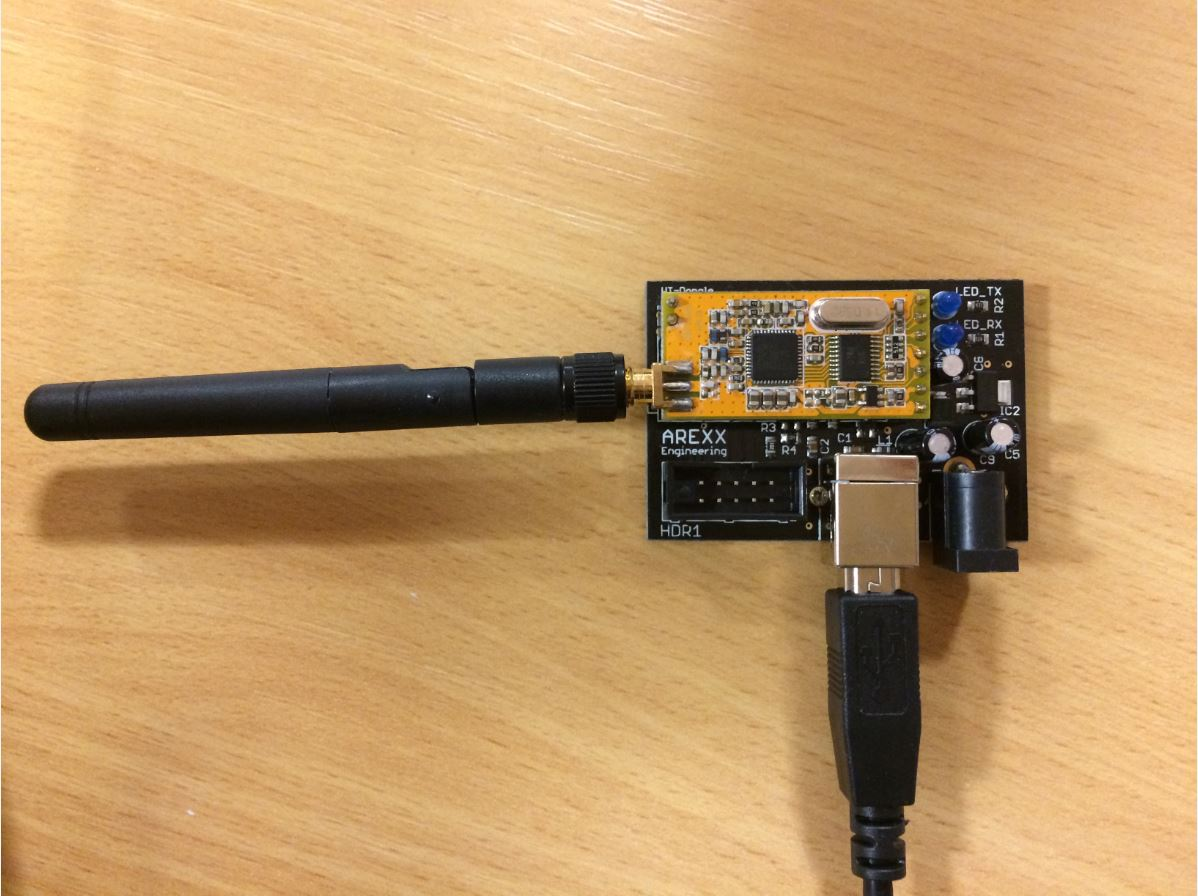
\includegraphics[scale=0.50]{ttlinterface_low}
\caption{UART/TTL Interface}
\label{fig:ttlinterface}
\end{center}
\end{figure}

The servomotors on the arm are controlled through the use of an Atmel ATMEGA64 8-bit Microcontroller, interfaced through a custom PCB designed by \textbf{AREXX} (full circuit diagrams available in Appendix). The microcontroller is based on the \textbf{AVR} architecture, architecture that has become widespread since its usage in the popular \textbf{Arduino} platform. It features EEPROM storage, allowing permanent storage of any AVR program, until it is overwritten. The platform benefits from an available suite of development tools, allowing compilation from \textbf{C} and \textbf{C++}, called WinAVR.

The Robotic Arm will be attached to the side of the robot body, as seen in \textbf{Figure \ref{fig:robotarm_attached}}.

\begin{figure}[H]
\begin{center}
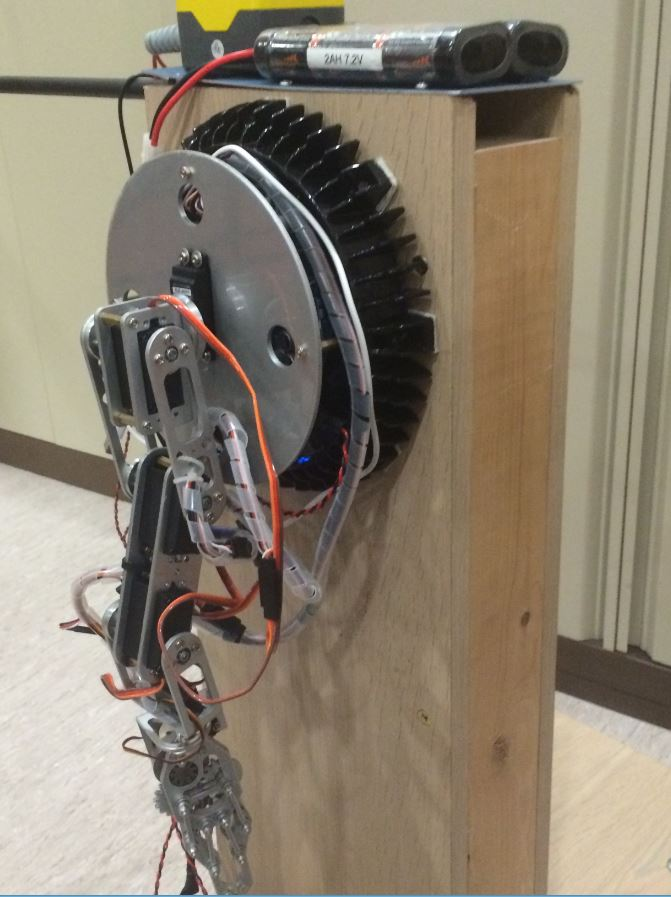
\includegraphics[scale=0.50]{robotarm_attached_low}
\caption{Robot Arm attachment to Structure}
\label{fig:robotarm_attached}
\end{center}
\end{figure}

\subsection{Sensors and Structures used for Retrieving Joint Parameters}

For controlling the arm, a natural interface will be devised in order to provide control through natural movements. The goal will be to make the robotic arm mimic the user's right arm. 
A combination of different technologies will be required for effective control. 
\subsubsection{Kinect V1/V2}

Several tests have shown that the Kinect is not precise enough to track wrist movements. It is however an ideal solution for tracking shoulder and elbow movements, due to it being markerless and reasonably precise.

\subsubsection{Leap Motion}

The \textbf{Leap Motion} is an optical based markerless hand-tracking device, measuring in at just (79 x 30 x 11mm) (\textbf{\ref{fig:leapview}}). It has the ability to track all 10 fingers simultaneously, including the bones forming the fingers, and it exposes all this information through its API. The interface used is a standard USB2.0 interface.

The Leap Motion compensates the Kinect extremely well, since the Kinect is not able to track the fine movements performed by the human hand, whilst the Leap is extremely proficient at it.

\begin{figure}[H]
\begin{center}

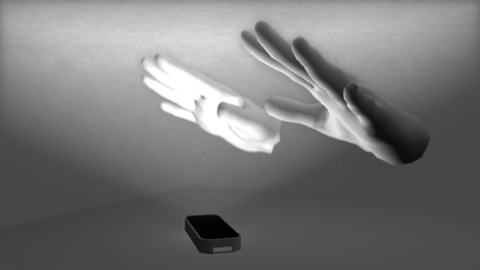
\includegraphics[scale=0.70]{Leap_View}
\caption{The Leap Motion controller’s view of your hands}
\label{fig:leapview}
\end{center}
\end{figure}

The main drawback of the Leap is its highly limited range of operation, being able to track at distances in-between \textbf{25 to 600 millimeters}.

As such, the user's hands have to be placed above the Leap at all times in order to allow for tracking. In order to provide the user with freedom of movement, a structure will have to be devised that will maintain the relative distance between the Leap and the hand constant, irrespective of where the user's arm is.

The structure will need to be attached to the base of the user's forearm, since:

\begin{itemize}
\item Attachment to the forearm makes the relative position of the Leap impervious to shoulder and elbow movements.
\item The \emph{pronator teres} muscle, responsible for pronating (anatomical rotation) the forearm and hand, extends from the base of the forearm. The amount of rotation the forearm is subjected to is minimal at the base, and increases over the length of the muscle. Thus, since the goal is to make the Leap impervious to this type of rotation (thus allowing tracking of wrist rotation), the structure needs to be attached to the base of the forearm.
\end{itemize} 

\begin{figure}[H]
\begin{center}
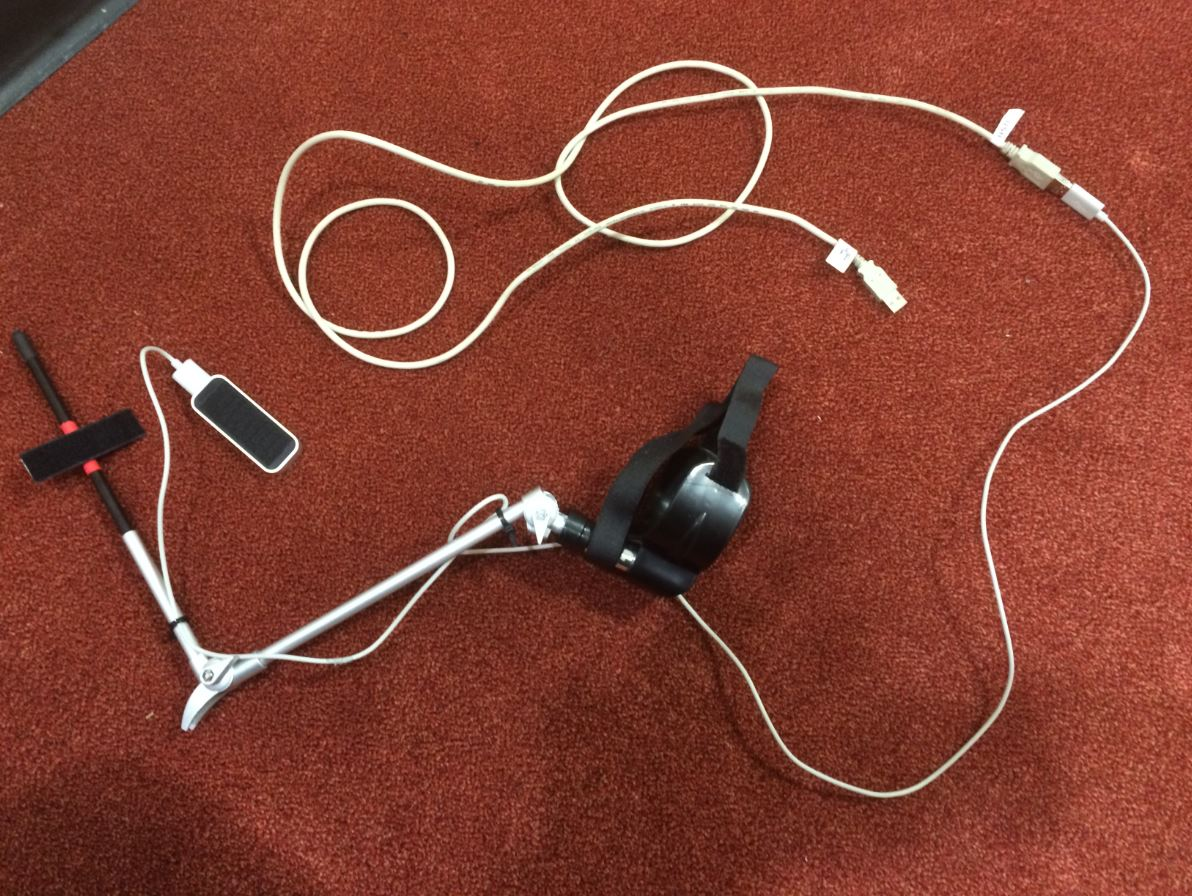
\includegraphics[scale=0.50]{leap_support_structure_low}
\caption{Leap Support Structure that attaches to the forearm. Extension USB cable needed to allow for increased freedom of movement.}
\label{fig:leap_support_structure}
\end{center}
\end{figure}

The structure depicted above, in \textbf{Figure \ref{fig:leap_support_structure}}, has been constructed in order to provide the requirements previously outlined. It presents a cuff at the top that wraps around the base of the forearm, as well as additional velcro straps that provide increased stability. The base is linked to a rod, which has two degrees of freedom, being able to flex up and down, as well as rotate. The first rod is then connected to a second rod through a joint which provides an additional degree of freedom, being able to flex up and down.

The second rod presents a small, metallic plate, that can glide up and down, as well as rotate around its center point. This confers another two degrees of freedom. 

The Leap Motion is attached to the metallic plate through two velcro strips. The flexibility of the structure allows the Leap to be perfectly positioned underneath the human hand at all times, being impervious to movements that need to be ignored.  

\begin{figure}[H]
\begin{center}
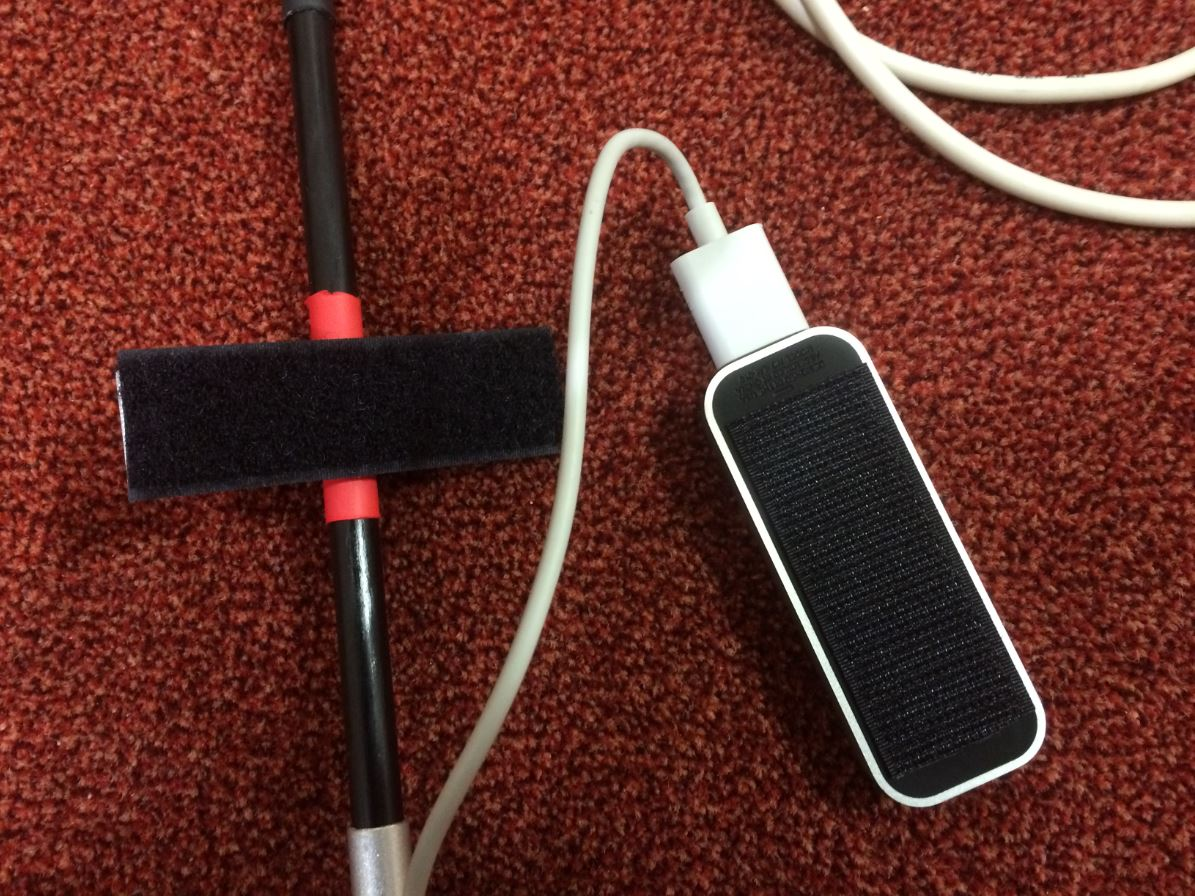
\includegraphics[scale=0.50]{leap_velcro_low}
\caption{The Leap, being able to attach itself to the metallic plate through the use of Velcro.}
\label{fig:leap_velcro}
\end{center}
\end{figure}

\subsection{Control}

Both the \textbf{Kinect} and the \textbf{Leap Motion} will be connected through USB to a computer. The computer will carry out the required computations required for determining the appropriate configuration for the robotic arm, and it will relay these over through the \textbf{USB to UART/TTL} converter depicted in \textbf{Figure \ref{fig:leap_velcro}}.

\newpage
\section{Movement Assembly}

The \textbf{Movement Assembly} will consist of all the hardware and software components that will allow the user to control the locomotion of the robot.  
\subsection{Glove Design}
For locomotion control, \textbf{an inertial system} will be used, achieved through the means of an accelerometer/gyroscope sensor, attached to the user's left arm, by means of a glove.

The required electronics will be sewed into the glove, and the orientation of the hand will be transmitted wirelessly to a microcontroller located on the moving assembly.

There glove will comprise of five components (See \textbf{Figure \ref{fig:glove_diagram}} for circuit diagram and \textbf{Figure \ref{fig:glove_component}} for implementation result):

\begin{itemize}
\item \textbf{Accelerometer/Gyroscope Sensor} - For the purpose of this project, the \textbf{MPU-6050} will be used. The MPU-6050 interfaces with the Arduino using an I \textsuperscript{2}C interface, which operates using two lines, a clock line (\textbf{SCL}) and a data line (\textbf{SDA}) \cite{i2c}. 
\item \textbf{Microcontroller} - A small microcontroller is required, so as to not restrict movement in any way. An \textbf{Arduino Pro Mini 328 - 3.3V/8MHz} has been chosen.
\item \textbf{Transceiver} - Required in order for the microcontroller to send sensor readings wirelessly to the moving assembly. An \textbf{XBee module}, alongside a shield have been chosen due to ease of implementation and extensive documentation found online.
\item \textbf{Power Source} - Power is provided by four AAA batteries, providing a total of 6V. All components benefit from having built-in voltage regulators, capable of regulating 6V to either 5V or 3V.
\item \textbf{Power Switch}
\end{itemize}



\begin{figure}[H]
\begin{center}
\makebox[\linewidth]{
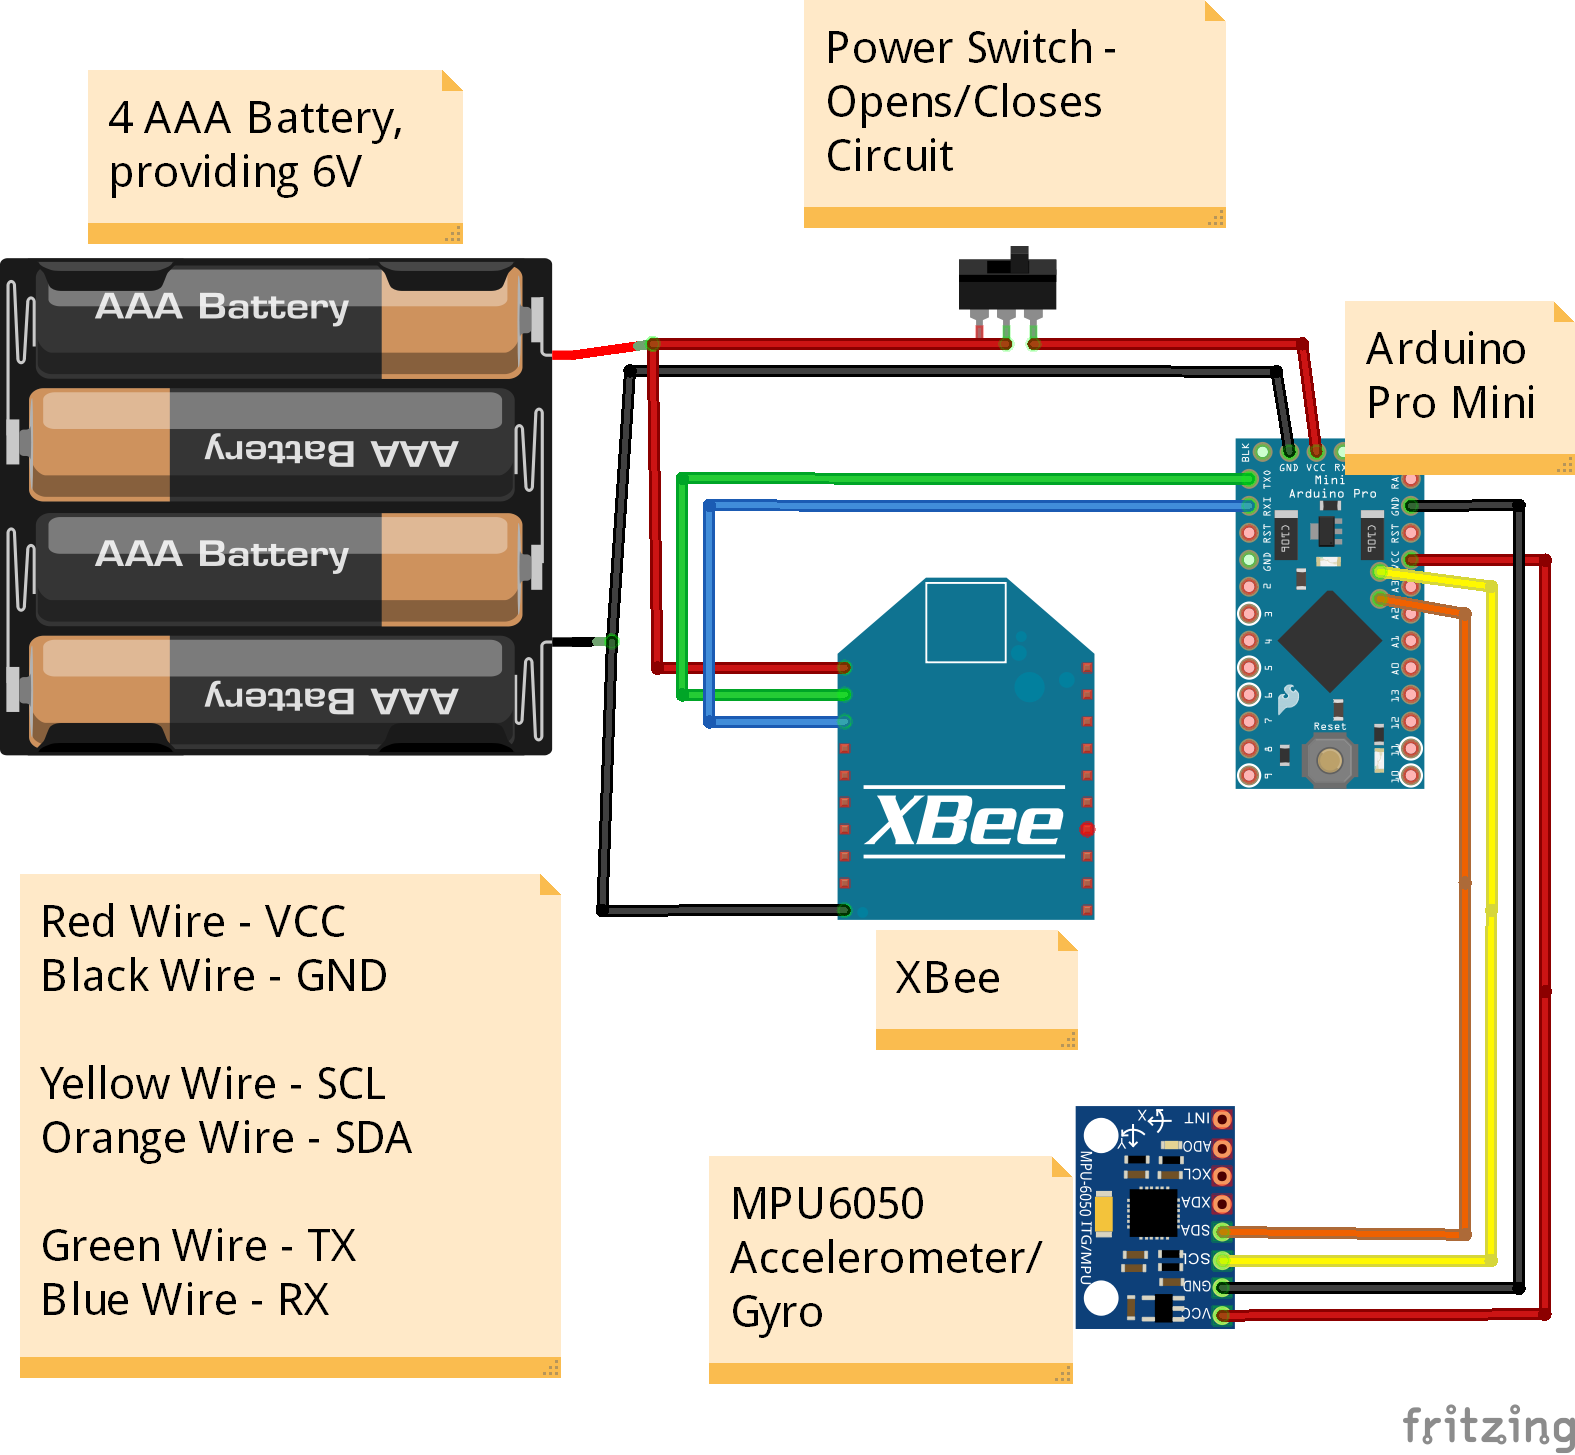
\includegraphics{glove_diagram2}
}
\caption{Glove circuit outline}
\label{fig:glove_diagram}
\end{center}
\end{figure}

\begin{figure}[H]
\begin{center}
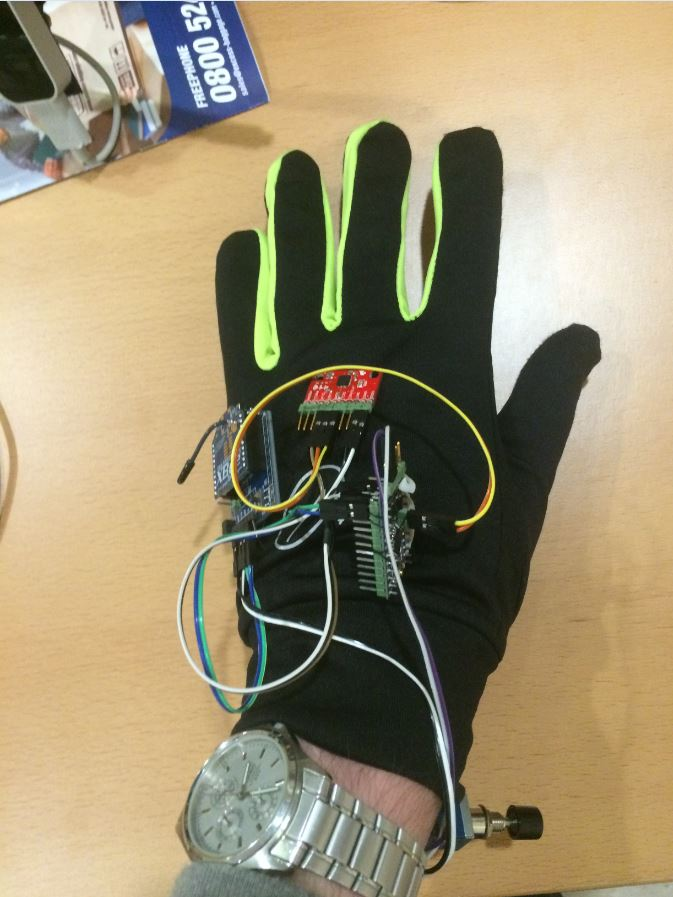
\includegraphics[scale=0.50]{glove_component_low}
\caption{Depiction of the glove used for locomotion control.}
\label{fig:glove_component}
\end{center}
\end{figure}

\subsection{Wheeled Locomotive Assembly Design}

Given the need for precise movement and the ability to steer, we will disregard non-wheeled locomotion. For steering, we will use a \textbf{differential steering mechanism}, due to both its ease of implementation as well as versatility.

For the purpose of this project, the \textbf{Rover 5 chassis} will be used, since it offers an adequate surface area as well sufficient motor torque. (\textbf{Figure \ref{fig:rover5}})

\begin{figure}[H]
\begin{center}
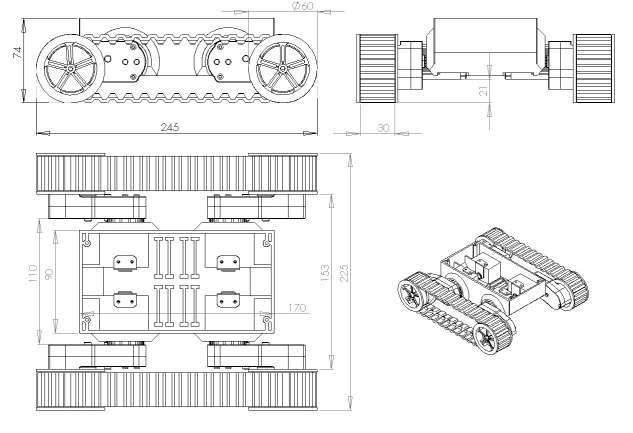
\includegraphics[scale=0.95]{rover5}
\caption{Rover 5 Size Specification \cite{rover5}}
\label{fig:rover5}
\end{center}
\end{figure}

The Rover 5 chassis has four DC motors, each responsible for powering a different wheel. Each pair of wheels drives a tread. The motors themselves take any voltage between -9V to +9V, the polarity indicating the direction of the spin. 


\textbf{Two} Rover 5 chassis will be used, each operating on either side of the robot. For each of the chassis, a metallic plate has been screwed on top, to which the main wooden structure is attached, through two screws on either side. For even balancing, a rubberized, pivoting nut is inserted between the two (Refer to \textbf{Figure \ref{fig:rover5robot}} and \textbf{Figure \ref{fig:rover5duo}} below).


\begin{figure}[H]
\begin{center}
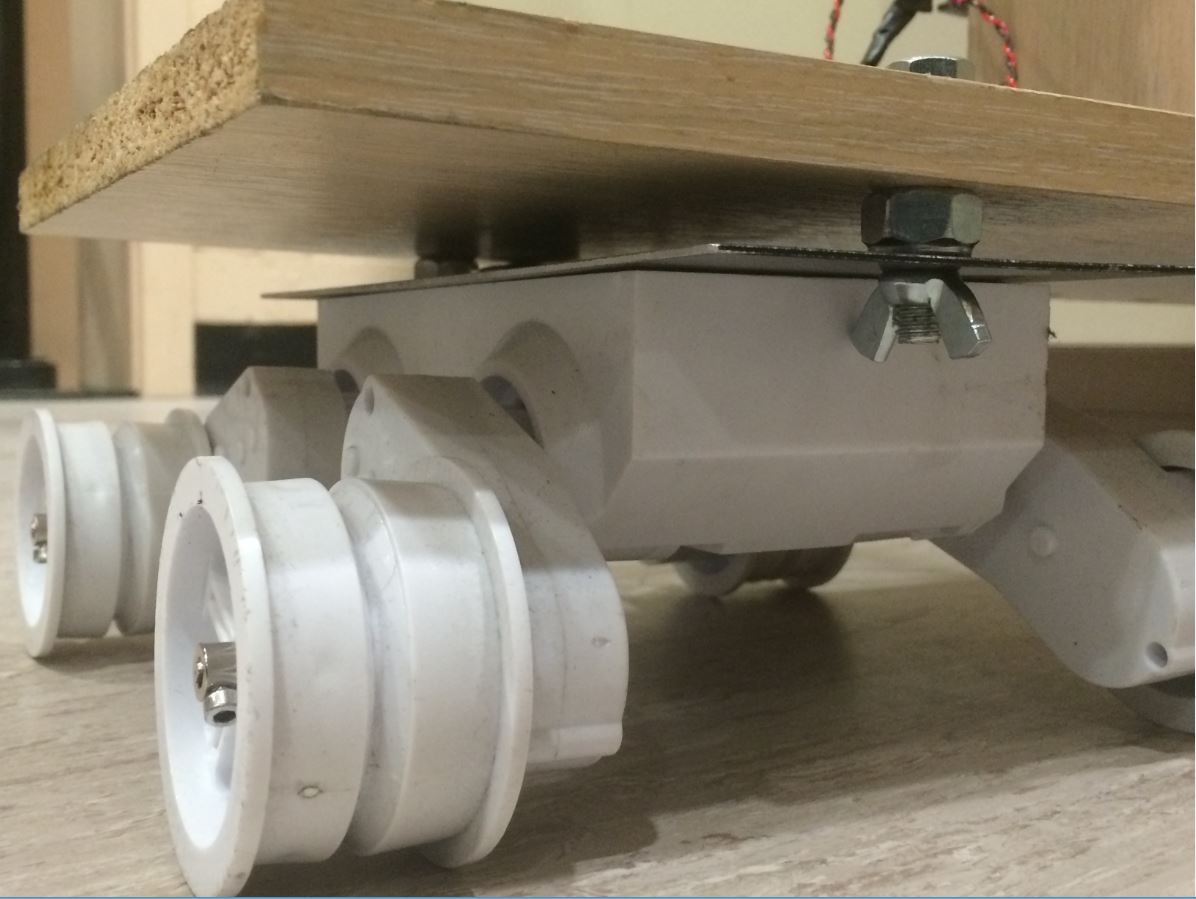
\includegraphics[scale=0.40]{rover5robot_low}
\caption{Movement Assembly Rover 5 Placement and Attachment}
\label{fig:rover5robot}
\end{center}
\end{figure}

\begin{figure}[H]
\begin{center}
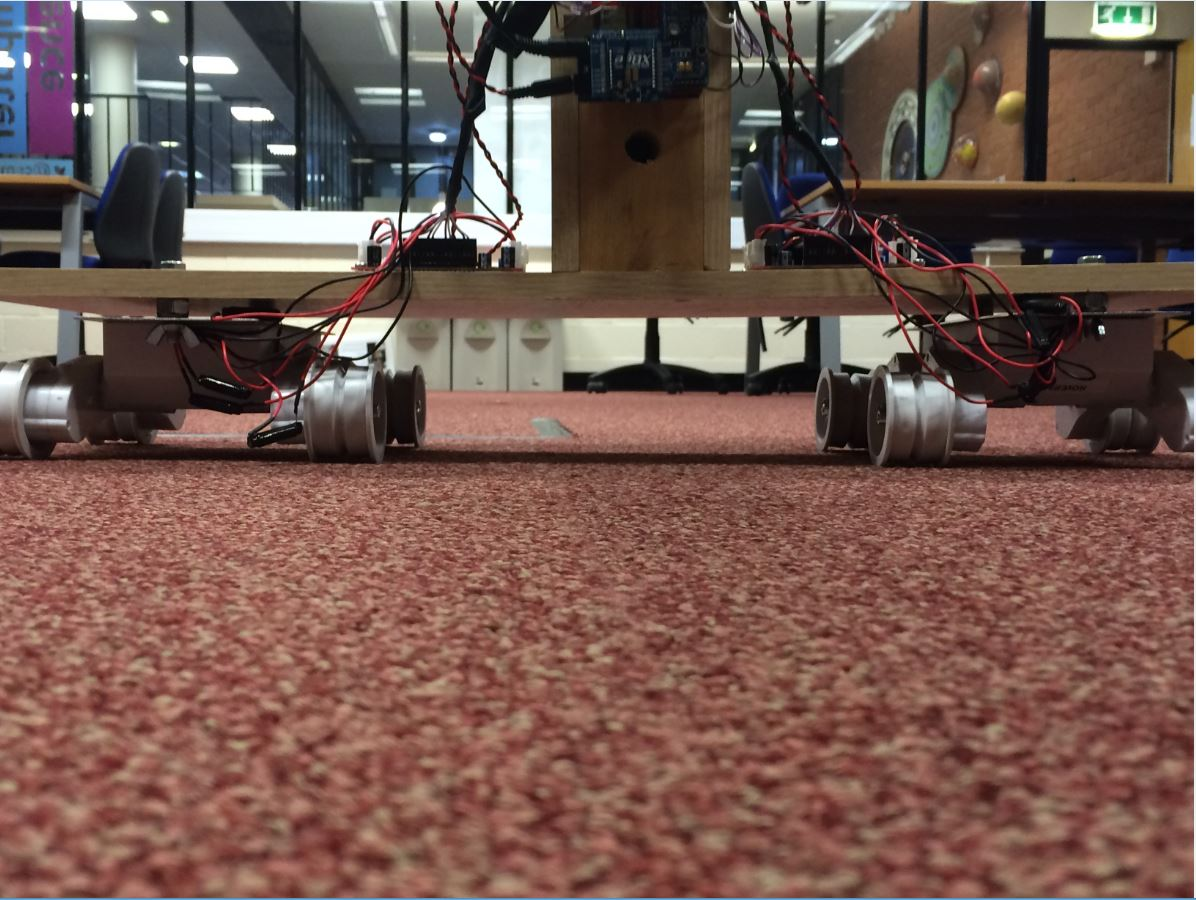
\includegraphics[scale=0.40]{rover5duo_low}
\caption{Robot Locomotion Assembly}
\label{fig:rover5duo}
\end{center}
\end{figure}
\newpage
\vspace*{-35pt}
Each Rover is connected to a Motor Driver board (See \textbf{Figure \ref{fig:movement_diagram}} for circuit diagram and \textbf{Figure \ref{fig:motordriver}} for implementation result), which regulates the voltage output using two input signals:

\begin{itemize}
\item a \textbf{PWM} signal, indicating the voltage (speed)
\item a digital \textbf{direction (DIR)} signal, indicating the polarity of the voltage (spin direction)
\end{itemize}

Even though each wheel can have its own PWM and DIR, the signal cables will be split 4-way, leading to all four motors on a rover, having each wheel move at the same speed and direction.

Additionally, for the purposes of this project, the PWM signal will be used to either specify a constant speed, or a full-stop (ignoring the benefits given by PWM).

Thus, only these scenarios will be supported:
\begin{itemize}
\item PWM Constant Speed: \begin{itemize}

\item \textbf{Forward Motion} - High Dir Signal for both Rovers
\item \textbf{Backwards Motion} - Low Dir Signal for both Rovers
\item \textbf{In-place left rotation} - High Dir Signal for Left Rover and Low for the other
\item \textbf{In-place right rotation} - Low Dir Signal for Right Rover and High for the other 

\end{itemize}

\item PWM Full-Stop:
\begin{itemize}
\item \textbf{No movement}.
\end{itemize}
\end{itemize} 
\begin{figure}[H]
\begin{center}
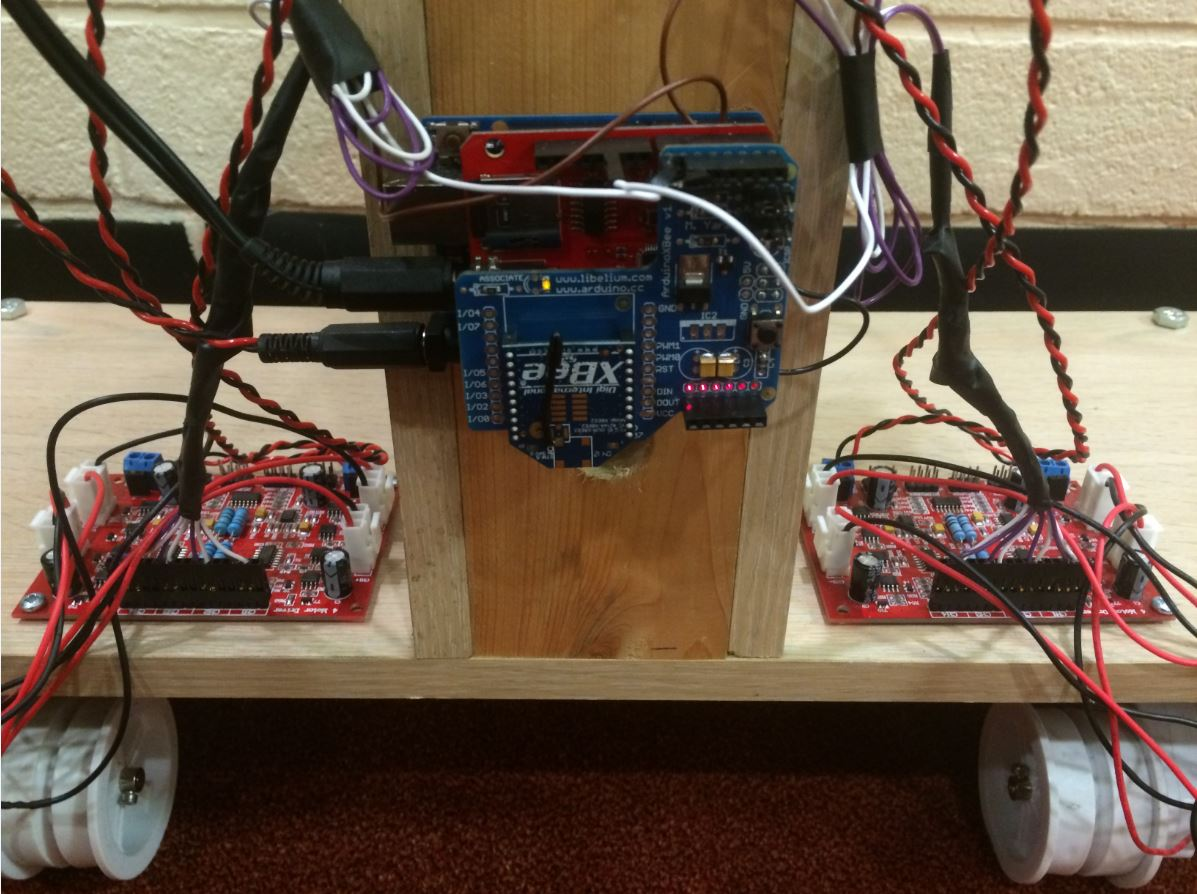
\includegraphics[scale=0.40]{motordriver_low}
\caption{Motor Drivers and Arduino Uno, as seen on the backside of the robot.}
\label{fig:motordriver}
\end{center}
\end{figure}


\begin{figure}[H]
\begin{center}
\makebox[\linewidth]{
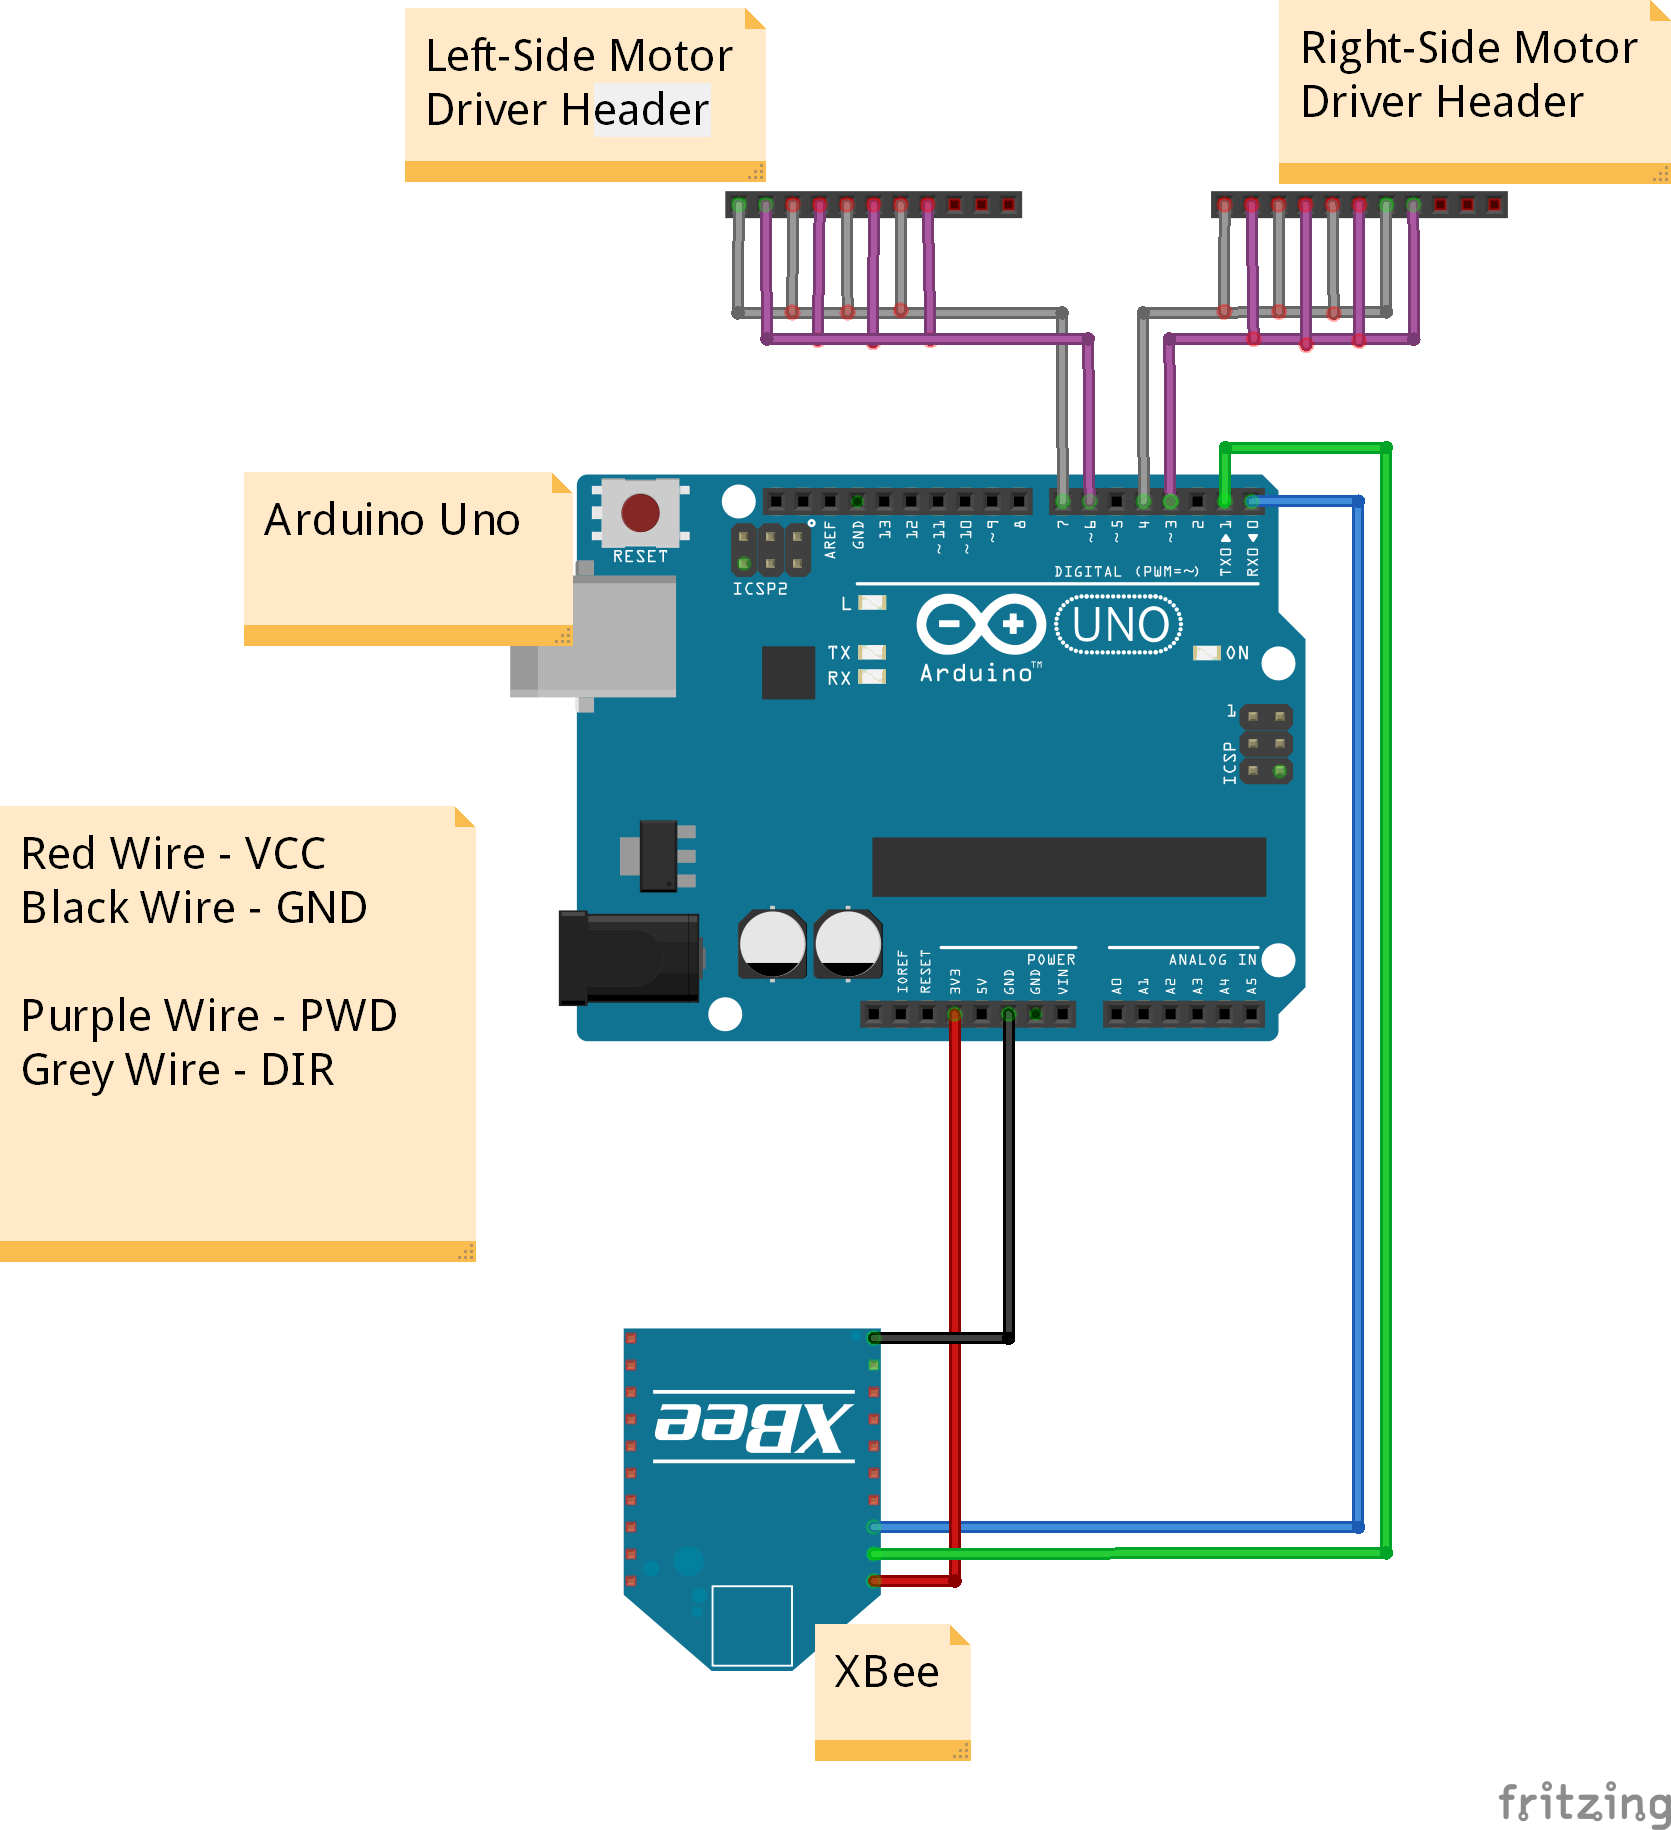
\includegraphics{movement_diagram}
}
\caption{Movement Assembly Circuit Overview}
\label{fig:movement_diagram}
\end{center}
\end{figure}


\section{Visual/Audio Feed and Telemetry Assembly}
In order to be able to guide the robot from a distance, details regarding its environment and the state of the robotic arm have to be relayed back to the operator. Most information needed for remote operation can be conveyed through a video and audio stream.


\subsection{Interface Details}
Relaying video and audio wirelessly, over large distance is not suitable for the serial interface discussed above due to bandwidth limitations. As such, a different communication protocol will be needed. For the purposes of this project, the \textbf{Internet Protocol suite} model will be used, since it provides virtually unlimited range if the connection is established through the \textbf{Internet}, as well as extremely high bandwidth capabilities.

In order to relay data wirelessly, an IPCamera could be used, since it incorporates the Wi-Fi capabilities needed. For the purposes of this project, an \textbf{IPhone 5S} will be used, since it can function as an IPCamera, being able to relay audio, and other data as well, since it contains a multitude of sensors (Magnetometer - Compass, Accelerometer, Gyroscope).

The phone is also able to emit light and/or sound, for long-range communication, or for lighting a dim room.

\subsection{Structure and Design}

An additional structure needs to be devised in order to attach the phone in a position that captures both what lies in front of the robot, as well as being able to capture the  configuration of the robotic arm.

The extension arm is attached orthogonally to the main structure. It is screwed in, whilst the phone is held in a tight grip by two plates. The configuration is adjustable, providing a good range of orientations for the phone to have.

\subsection{Oculus Rift Extension}

Optionally, an Oculus Rift can be used, such that it displays the streamed video coming in from the phone. This provides better immersion, as well as easing control of the robot.

\newpage
\section{Power Source and Voltage Regulation}
The power system needs to be designed such that it does not
hinder the mobility of the robot. \textbf{AC adaptors} will be used throughout the development and testing phase, since the platform does not need to be mobile in such instances, and there is no concern of draining a limited power supply. \\

There are several subsystems the power system will need to power:

\begin{itemize}
\item \textbf{RA1-Pro} - A voltage between \textbf{7-18V} is required, with current between \textbf{2 and 4Amps}.

\item \textbf{Rover 5 Motors} - A voltage of \textbf{9V} is expected.

\item \textbf{Rover 5 Motor Driver Board} - A voltage of \textbf{5V} is expected.

\item \textbf{Arduino UNO} - A voltage of \textbf{5V} is expected.

\item \textbf{Optional Speaker Amplifier} - A voltage of \textbf{5V} is expected.

\end{itemize}

In order to satisfy the above voltage requirements, we will make use of two, \textbf{Nimh Battery Pack SubC 2000mAh 7.2} batteries, proving a total of 14.4V and a capacity of \textbf{2000mAH}. An inline fuse has been added to the circuit, to prevent any damage in case of a short circuit.

Both batteries are attached to the top of the structure, through the use of velcro. (Top View of the robot viewable in \textbf{Figure \ref{fig:rover5power}}).


\begin{figure}[H]
\begin{center}
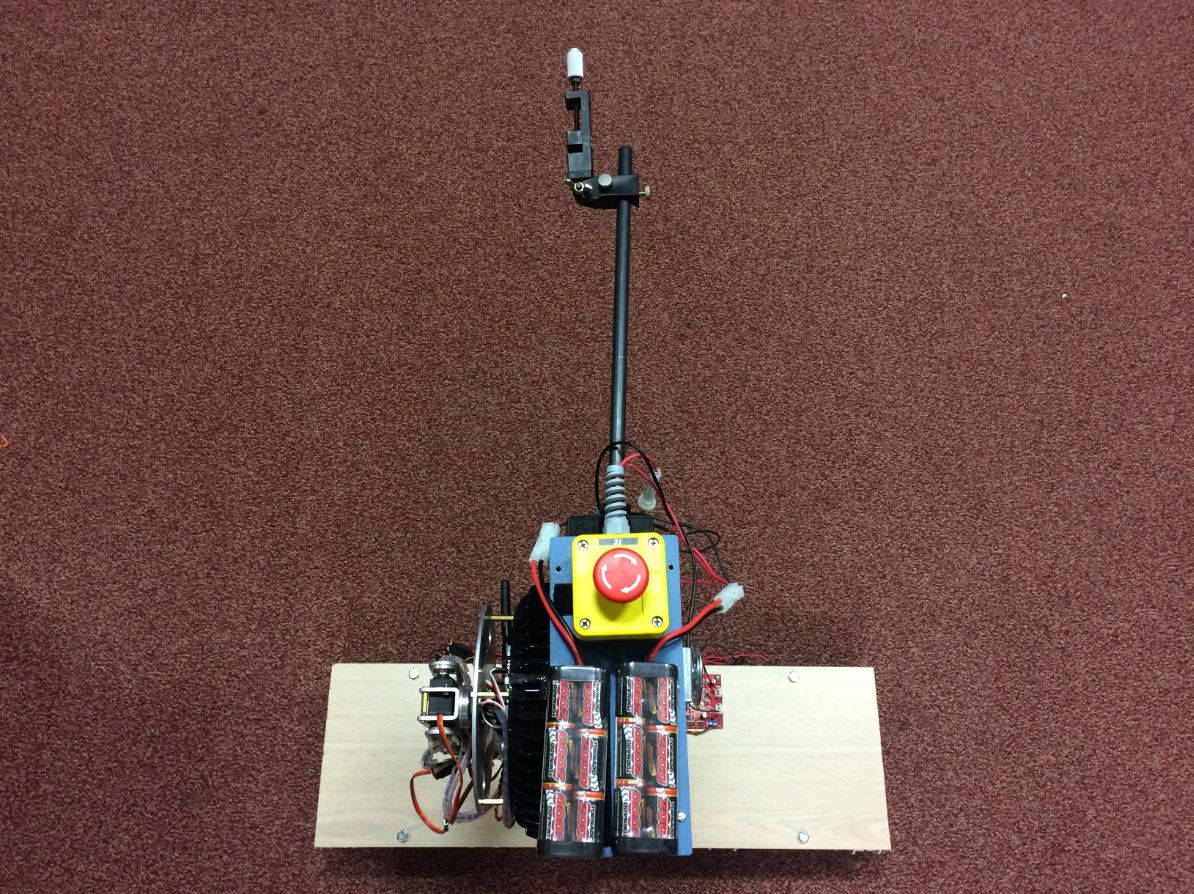
\includegraphics[scale=0.35]{power_source_low}
\caption{Power System, powering the various subsystems}
\label{fig:rover5power}
\end{center}
\end{figure}

The battery is connected through the means of a \textbf{circuit switch}, taking the form of a red button. It can serve to either shut down the system in order to save battery, or as a kill switch to interrupt unexpected behavior.

The current is then fed, in series, through three \textbf{voltage regulators}, for \textbf{12V, 9V and 5V} respectively. Observations suggest a battery life expectancy between 20-30 minutes with all subsystems being operational (See \textbf{Figure \ref{fig:voltageregulators}}). 
\begin{figure}[H]
\begin{center}
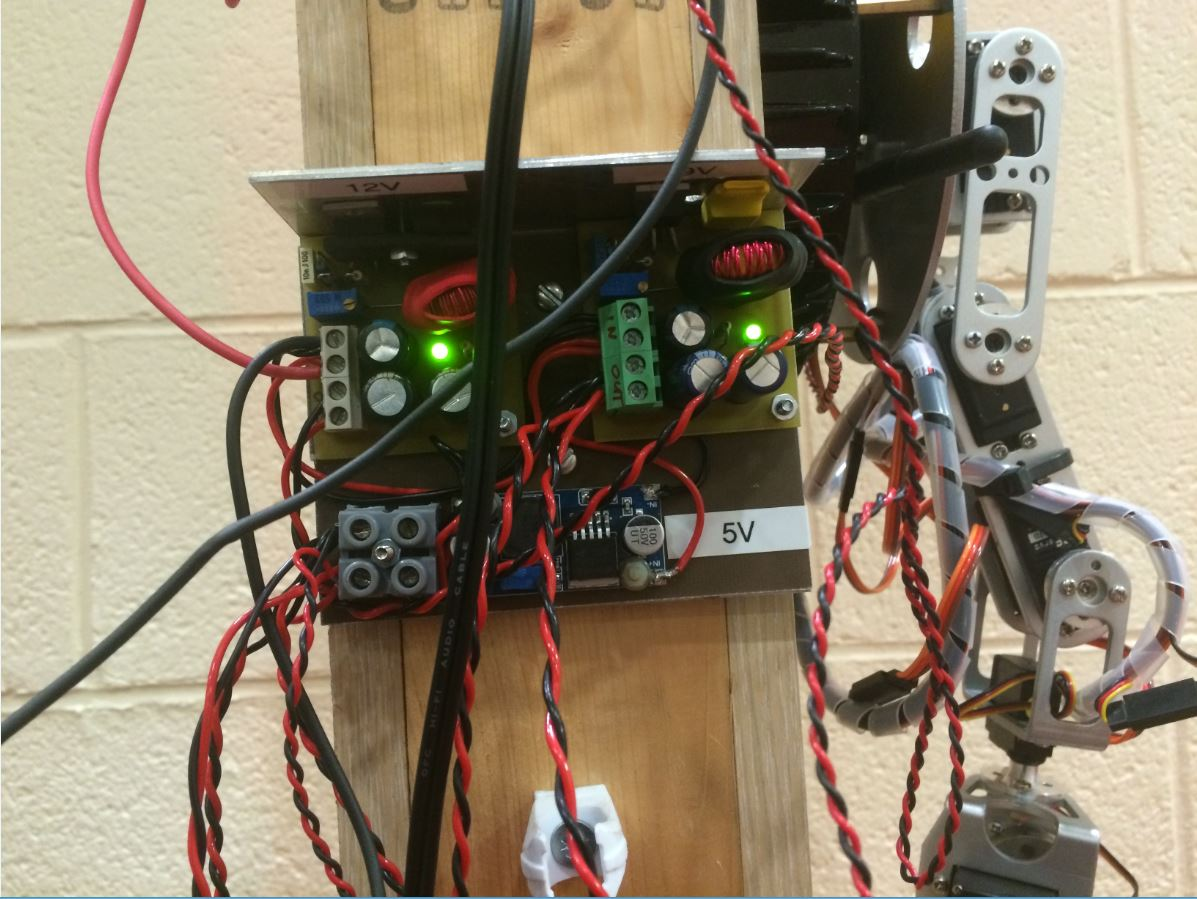
\includegraphics[scale=0.50]{voltage_regulators_low}
\caption{5V, 9V and 12V regulators, powering the various subsystems}
\label{fig:voltageregulators}
\end{center}
\end{figure}



\begin{figure}[H]
\begin{center}
\makebox[\linewidth]{
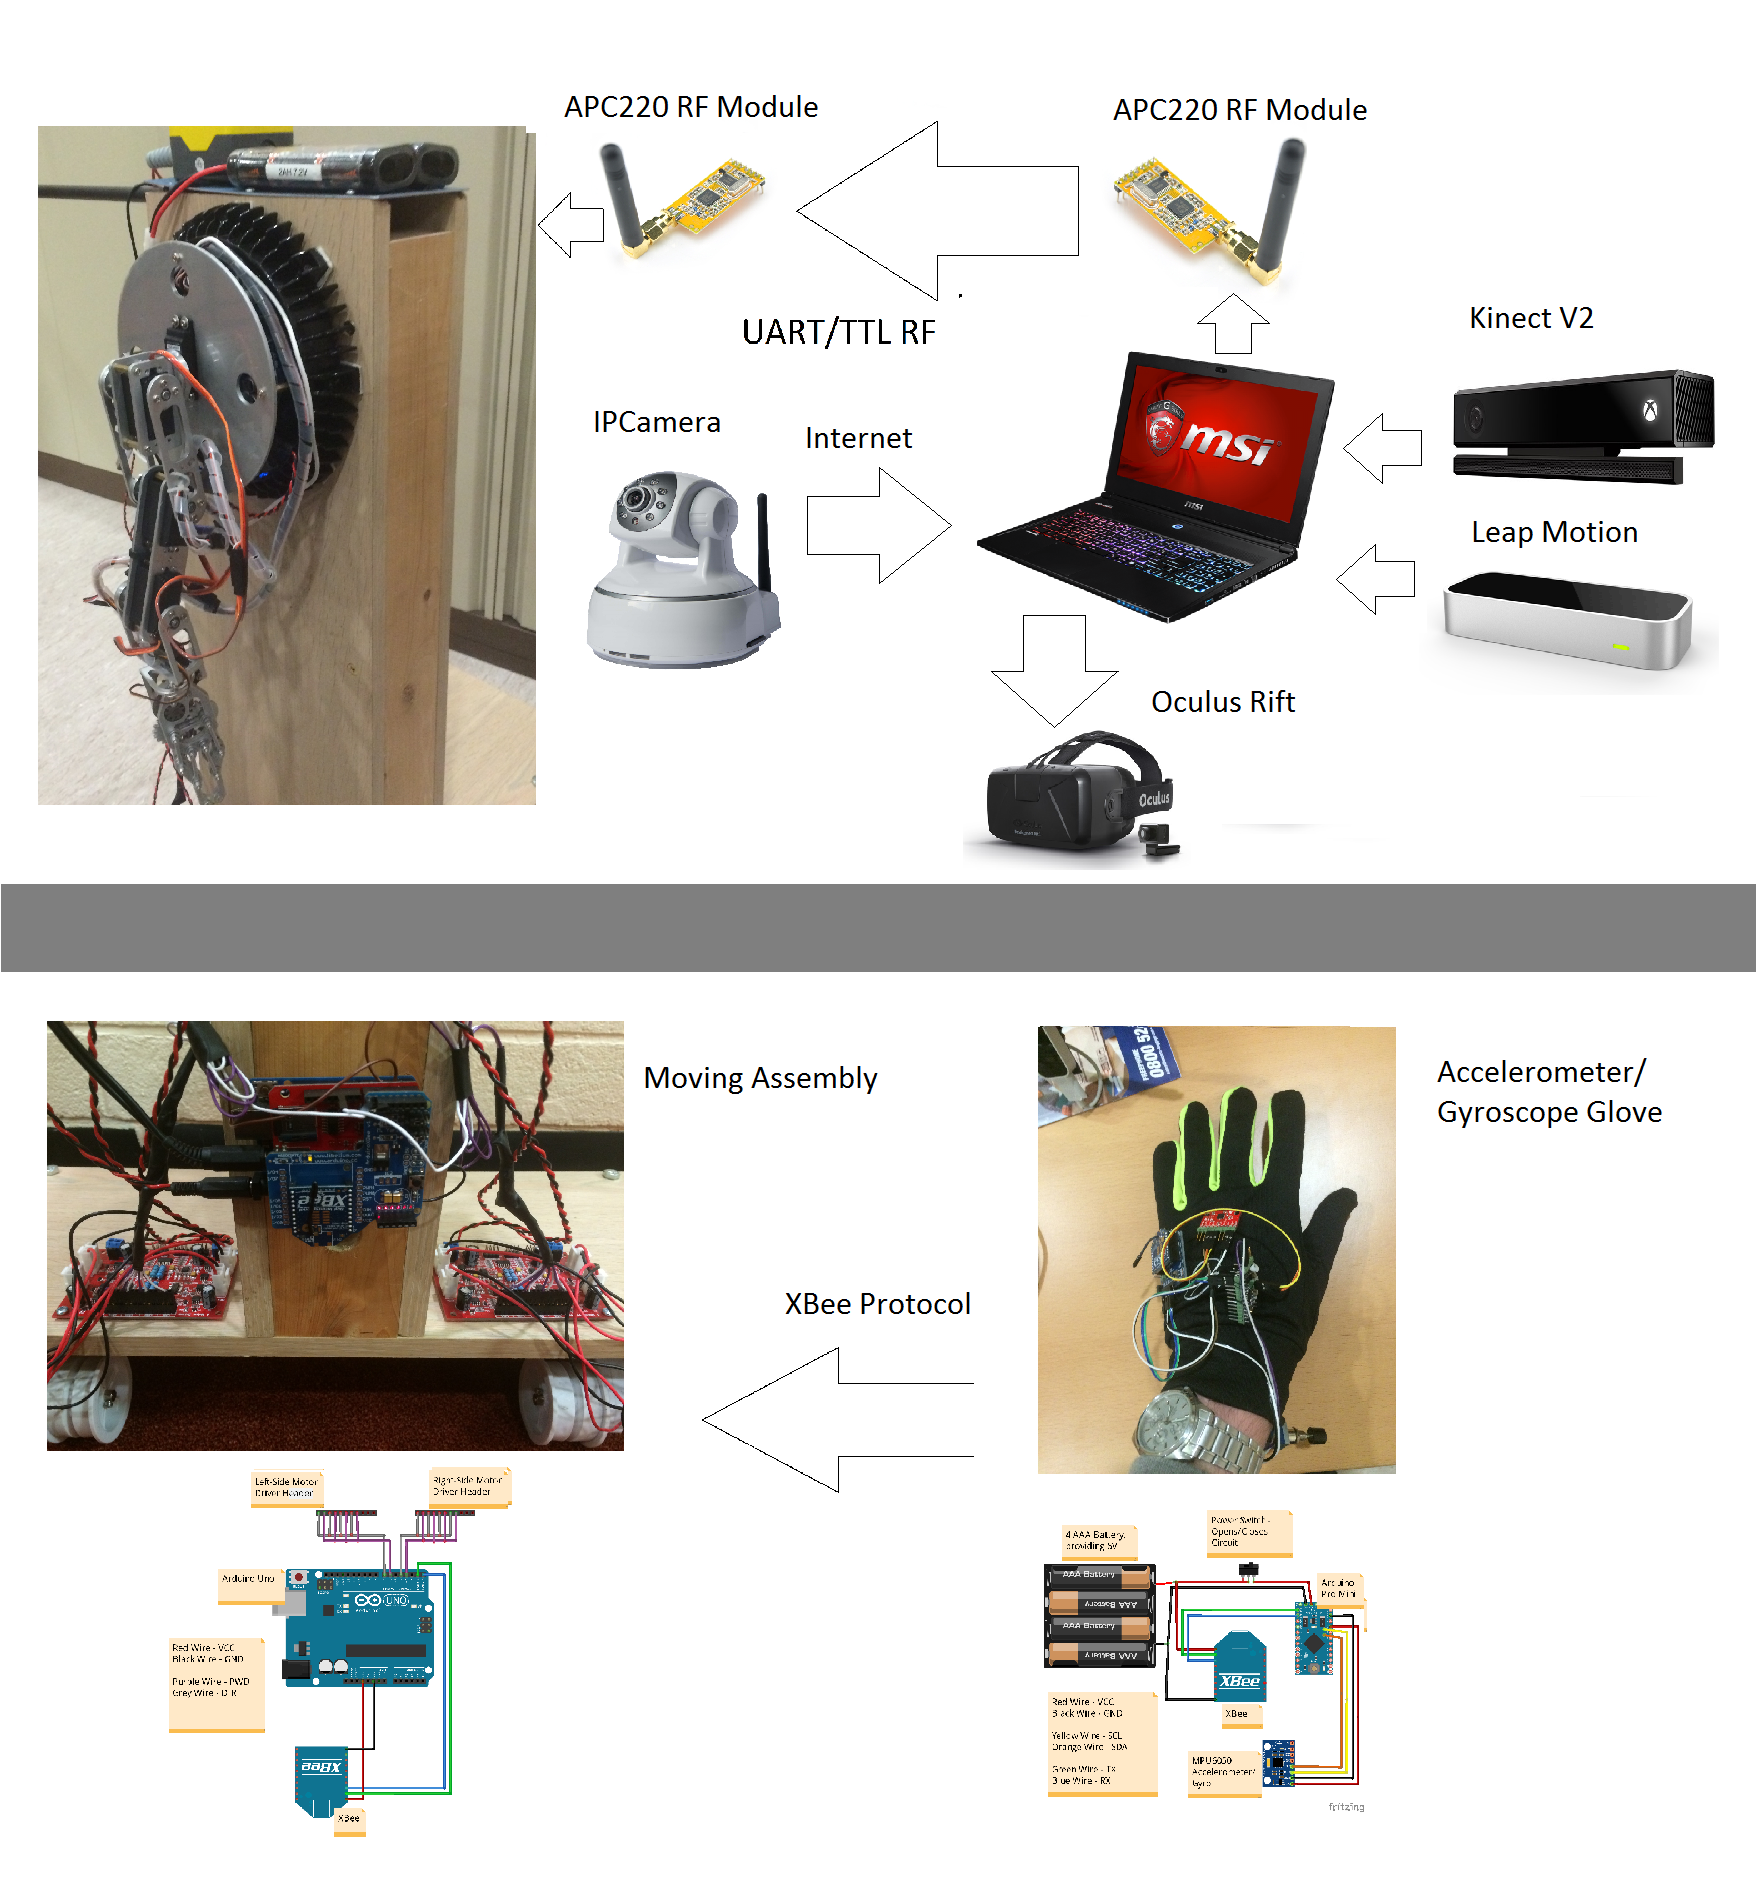
\includegraphics[scale=0.4]{overall_schematic3}
}
\caption{Overall Design Schematic - Note the two independent components, separated by the grey border.}
\label{fig:overall_schematic}
\end{center}
\end{figure}


\chapter{Software Development}
This chapter will cover both the design and the development of the software required to make the robot operational. Due to the nature of the hardware involved, the various number of interfaces used, and the different degrees of computation power needed to perform tasks, the software evolved into two, independent components. 


\section{Robotic Arm Software Platform}

Parameters for the Robotic Arm are computed on a computer, and related wirelessly through the USB to UART/TTL interface described above. The computer computes these parameters making use of both the Kinect and Leap Motion, to which its connected to.

\subsection{Language and Technologies Chosen}

The \textbf{.NET} platform has been chosen, due to ease of integration with the Kinect and Leap. \textbf{C\#} has been selected as the language of choice, due to the \textbf{Windows Presentation Foundation (WPF)} framework built on top of it, which provides convenient tools for creating a viable user interface.  
\newpage
\subsection{Robot Arm Serial Communication}

Communication to the arm is done using a library for \textbf{COM} communication (serial devices). A baud rate is set, relaying the configuration of the arm at regular intervals.

The arm's microcontroller operates at the same baud rate, receiving the commands from the computer and changing the configuration accordingly. The arm's microcontroller program that was used was provided by the arm's manufacturer, \textbf{AREXX}.


\subsection{Determining End-Effector Parameters using the Leap API}

The Leap API provides a very easy method for determining several parameters relating to the hand. For the purpose of this project, roll and pitch will be used to rotate and flex the end-effector, and \textbf{pinch strenght} will be used for determining the gripper's configuration.

\begin{verbatim}
pinchStrength = frame.Hands.Count > 0 ? frame.Hands[0].PinchStrength:pinchStrength;
wristPitch = frame.Hands.Count > 0 ? frame.Hands[0].Direction.Pitch:0;
wristRoll = frame.Hands.Count > 0 ? frame.Hands[0].Direction.Roll : 0;
\end{verbatim}
\subsection{Determing Joint Parameters using the Kinect API}

The robotic arm actuators will be set such that the angles between each of the joints will correspond to the angles formed between the joints in a human arm.

The Kinect API provides Skeleton tracking information, allowing for easy retrieval of Joint data (See \textbf{Figure \ref{fig:kinectbody}} for available joints). 

\begin{verbatim}
// Returns information pertaining to the ShoulderCenter joint
jointCollection[JointType.ShoulderCenter]
\end{verbatim}

\begin{figure}[H]
\begin{center}
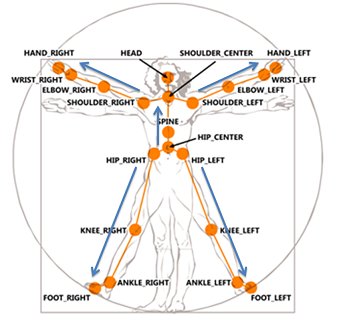
\includegraphics{kinectbody2}
\caption{Kinect Skeleton Representation \cite{mocapsports}}
\label{fig:kinectbody}
\end{center}
\end{figure}

Each Joint object has \textbf{x, y, z} coordinates. This information is then used in order to compute an angle between any three, consecutive joints.

This is a trigonometric problem, which reduces to two steps (See \textbf{Figure \ref{fig:angle}}):

\begin{itemize}
\item Use the 3 points to create two vectors $\overrightarrow{J2J1}$ and $\overrightarrow{J2J3}$ \\
$
\overrightarrow{J2J1} \langle x1 -  x2, y1 - y2 \rangle 
$ \vspace{5pt} \\
$
\overrightarrow{J2JJ3} \langle x3 -  x2, y3 - y2 \rangle
$


\item Compute the angle between the two vectors \\

$atan2(J2J1.y, J2J1.x) - atan2(J2JJ3.y,  J2JJ3.x)
$ \\

This will return a result in radians, in the range of $(-\pi,+\pi)$

The range will be changed in order to better describe the angles. We will begin by adding $\pi$, thus, translating the range to $(0,+2\pi)$. We will then convert the radians to degrees, by multiplying with $\frac{180}{\pi}$.

\end{itemize}

\begin{figure}
\begin{center}
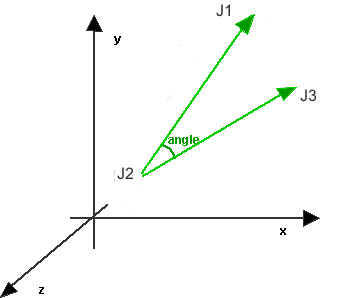
\includegraphics{angle}
\caption{Angle corresponding to J2}
\label{fig:angle}
\end{center}
\end{figure}

In order to minimize noise, the user can choose to sample the range of possible joint angles, having the real joint angle estimated as being the closest sample point. 

\begin{verbatim}
byte approximatedAngle = (byte)(Math.Round(newAngle / partitionSize) * partitionSize);
\end{verbatim}

\subsection{Visual Feed}
A visual feed is also provided by an \textbf{IPhone 5S} located on the robot, which acts as an IPCamera. The IPhone 5S runs an application called \textbf{IPCamera}, which hosts an HTTP server that it uses in order to relay a video feed taken from the camera, through the means of a web page. If both the computer and the IPhone are connected to the same network, the feed can be viewed from the computer, within a browser.

In order to integrate the feed within the WPF GUI, a framework will be used (\emph{Awesomium.NET}) that provides rendering of web pages pages within the application itself.

\subsection{GUI Design}
The \textbf{GUI} presents a simplistic design, being divided into four quadrants (See \textbf{Figures \ref{fig:userinterface}} and \textbf{\ref{fig:userinterface2}}).

\begin{itemize}
\item \textbf{Top-Left Quadrant} - Displays the Skeleton view of the user through the use of the Kinect, showcasing the angles between various joints.
\item \textbf{Top-Right Quadrant} - Features Robot controls, allowing for connection, powering up servos, as well as controlling the position of each servo through a slider. If the checkbox on the left side of a specific joint is ticked, input will be taken from the corresponding motion capture device.
\item \textbf{Bottom-Left Quadrant} - Displays the Leap's view of the hand, showing values for Roll, Pitch and Yaw, as well as the Pinch Strength.
\item \textbf{Bottom-Right Quadrant} - Displays the Visual feed, received from the camera attached to the robot (the IPhone 5S).
\end{itemize}


\begin{figure}[H]
\begin{center}
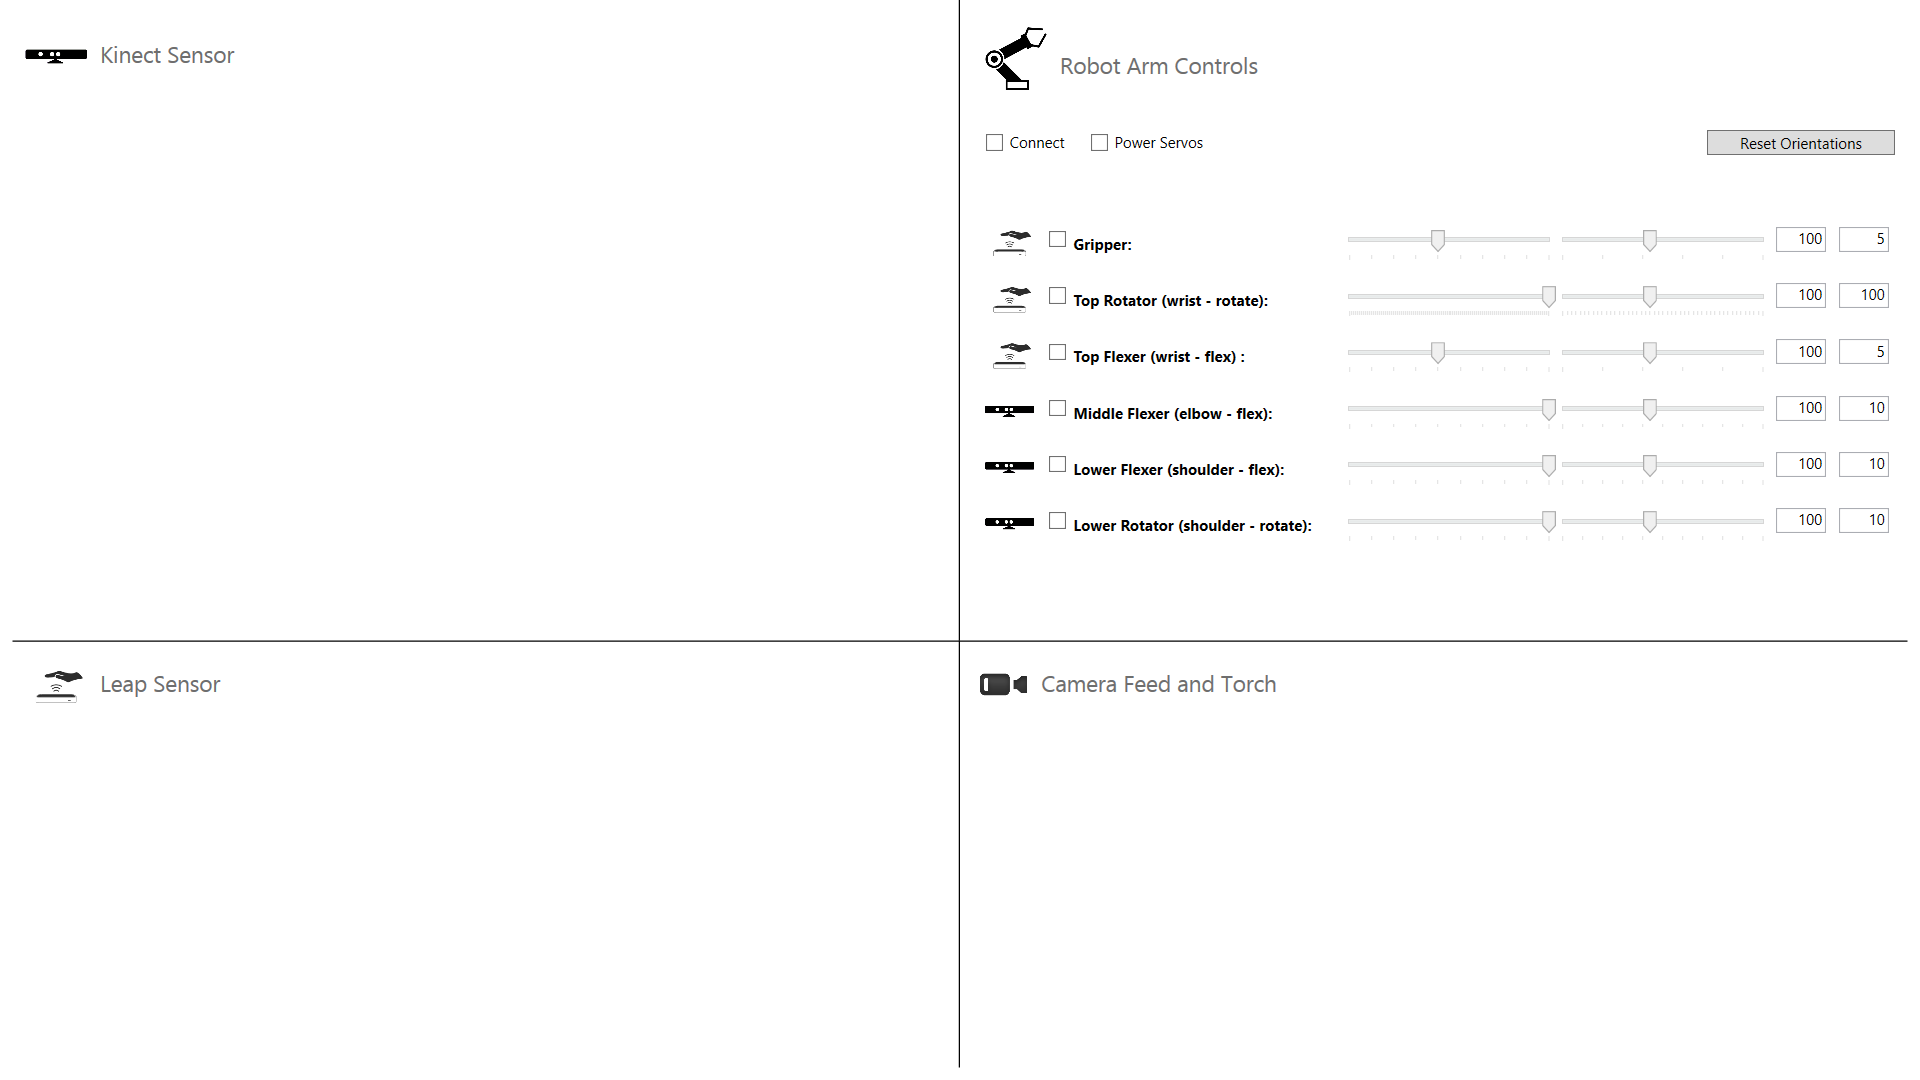
\includegraphics[scale=0.3]{userinterface}
\caption{Robotic Arm WPF GUI}
\label{fig:userinterface}
\end{center}
\end{figure}


\begin{figure}[H]
\begin{center}
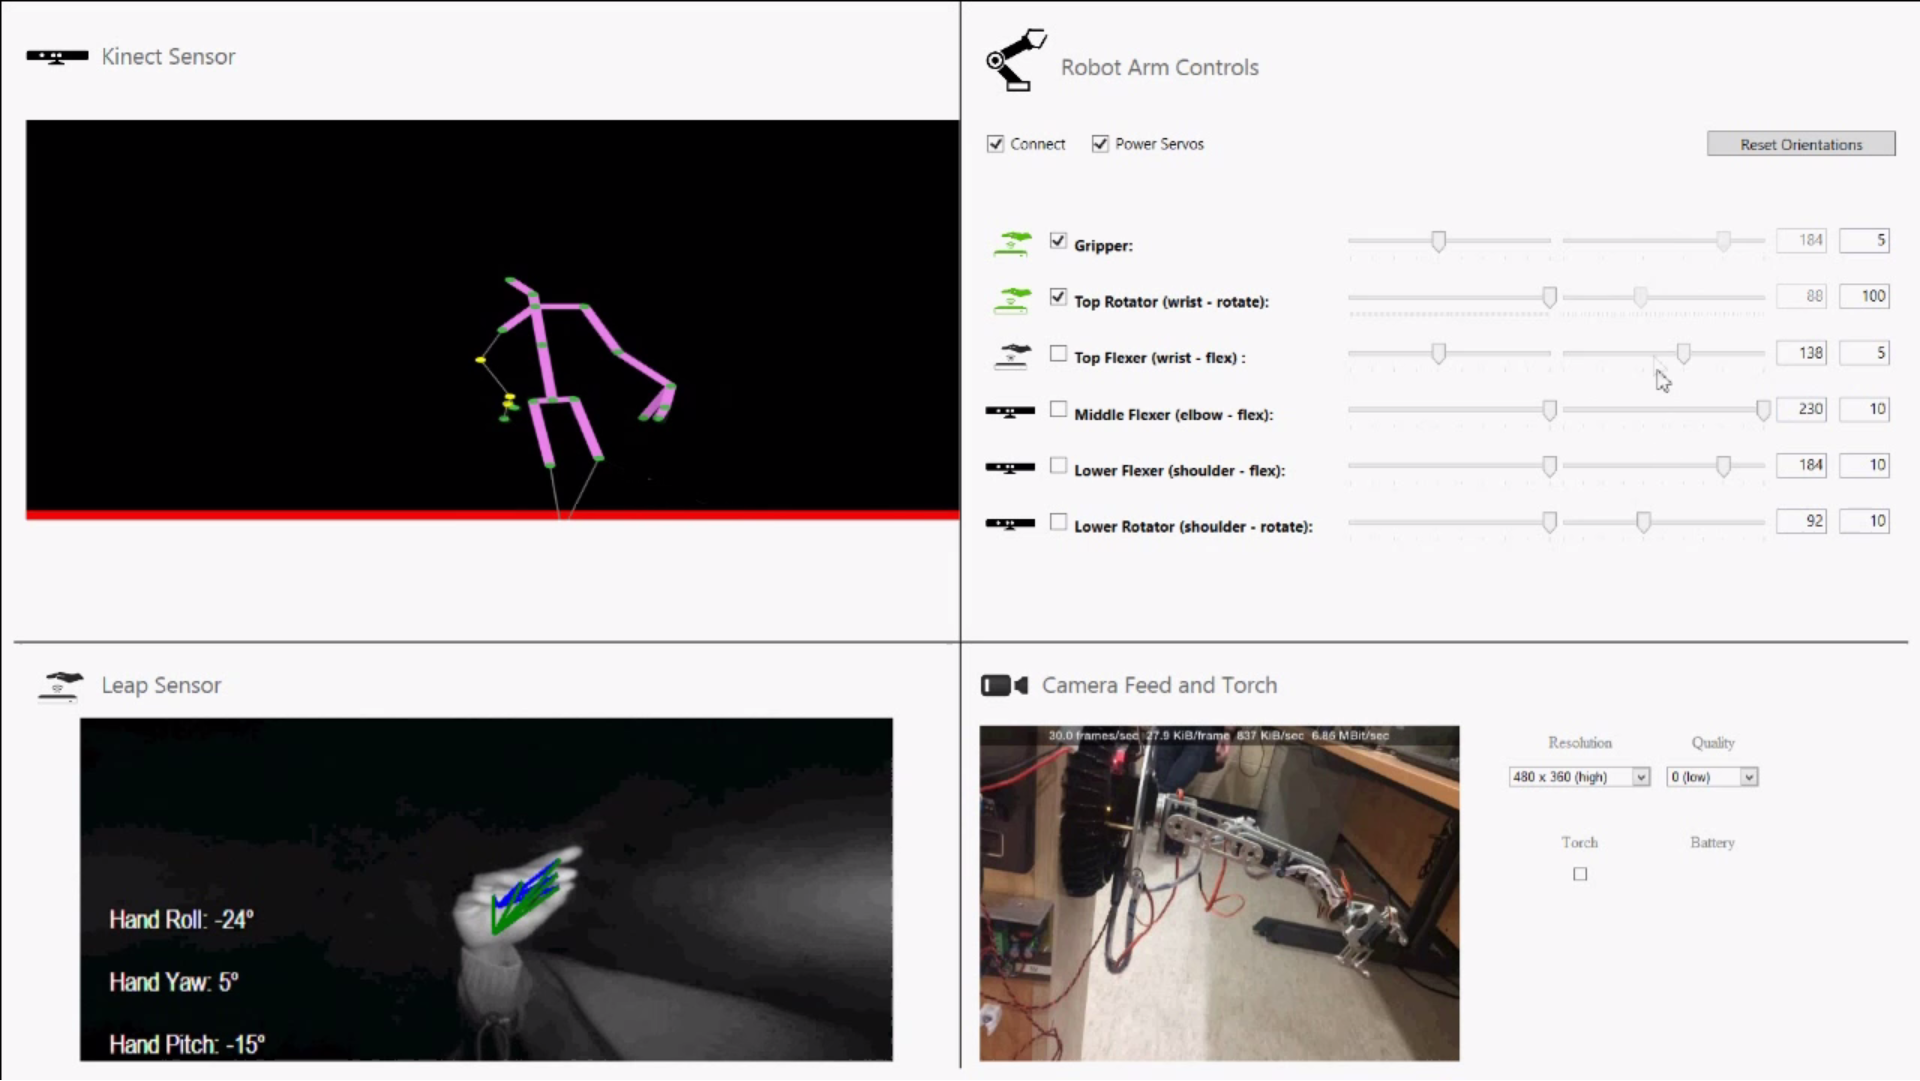
\includegraphics[scale=0.3]{userinterface2}
\caption{Robotic Arm WPF GUI}
\label{fig:userinterface2}
\end{center}
\end{figure}

\newpage
\section{Moving Assembly Software Platform}
In contrast to the Robot Arm software, all software for the moving platform is run on the two microcontrollers, located on the glove and the assembly.

The software is written in \textbf{C}, having two components, for the transmitter (located on the glove) and the receiver (located on the assembly).

Various Arduino C libraries exist, in order to allow easy interfacing with various components. The \emph{"MPU6050\underline{ }6Axis\underline{ }MotionApps20.h"} for instance, provides several methods for retrieving the sensor's roll, pitch and yaw. Once retrieved, a byte of information can be sent to the assembly, specifying the type of movement required.

\begin{verbatim}
if(roll > 50)
  Serial.print('F');
\end{verbatim}

Since the \textbf{TX} (write pin) of the Arduino is connected to the XBee, the byte will be sent to the XBee, getting packetized and relayed.

Once the XBee on the receiver intercepts the package, it will send it as output to the \textbf{RX} pin, being readable through the \textbf{Serial.read()} command. Once read, the appropriate signals are sent to the motor drivers, which set the appropriate voltages for each of the rover motors. 

\begin{verbatim}
  byteReceived = Serial.read();
  if(byteReceived == 'F')
  {
    analogWrite(LEFT_PWM, velocity);  
    digitalWrite(LEFT_DIR, HIGH);
    analogWrite(RIGHT_PWM, velocity);  
    digitalWrite(RIGHT_DIR, HIGH);    
  }
  else
    ...
\end{verbatim}
\chapter{Evaluation and Testing}
This chapter will explore the capabilities of the final product, as well as cover some testing carried out.

\section{Functionality and Accuracy}
Component-wise assessment:
\begin{itemize}
\item The power system is able to power the robot for up to 30 minutes under full-load conditions.
\item Locomotion wise, the robot presents precise control, with tested ranges of up to 100 meters. Due to it being wheel-based as well as having a high center of mass, it is only able to move across flat surfaces.
\item Arm control range is also up to 100 meters. Due to the noisy nature of the Kinect and markerless motion capture in general, very precise arm movements are hard to execute.  
\item Control is not very precise, due to the noisy nature of the Kinect and the Leap Motion.
\end{itemize}

\section{Testing}
Due to the heavy emphasis on hardware as well as on external API's, testing did not form a crucial part of this project. Hardware testing was done using a \textbf{multimeter} as well as schematics to ensure appropriate voltage and current to each of the components. 

There are two fundamental stages that required appropriate testing:
\begin{itemize}
\item \textbf{Motion Capture Testing} - Testing orientations and angles as provided by the various sensors and API's.
\item \textbf{Telecommunication Testing} - Testing whether the data was transmitted correctly to the required receiver.
\end{itemize}

Motion Capture for the Robotic Arm was done through the Kinect and Leap Motion API's, requiring little to no functionality on top. The trigonometric functions computing the angles between three joints have been subjected to \textbf{unit testing} throughout development.

Motion Capture for the Inertial Glove has been done by subjecting the sensor to various orientations and monitoring the byte that gets sent through the \textbf{Serial Monitor} tool, that is part of the Arduino IDE, as seen in \textbf{Figure \ref{fig:serialmonitor}}.


\begin{figure}[H]
\begin{center}
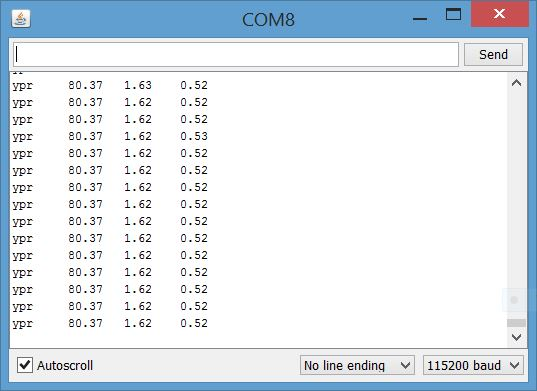
\includegraphics{serialmonitor}
\caption{Arduino Serial Monitor}
\label{fig:serialmonitor}
\end{center}
\end{figure}



Telecommunication Testing through both the UART/TTL interface, as well as the XBee, was done using several external libraries, requiring little additional testing.

At the end, \textbf{acceptance testing} has been carried out through the help of several volunteers, providing significant insight into means of improving control and the overall interface.

\chapter{Reflection and Conclusion}
\section{Issues Encountered}
Throughout the course of this project, there have been various iterations and issues encountered along the way.

\begin{itemize}
\item In its initial phase, the robotic arm was controlled through a  \textbf{wired} USB to UART/TTL interface. The interface proved to be defective, an issue which took three months to trace, delaying the progress of the project significantly.  

\item The \textbf{RA1-Pro} robotic arm came with low torque servomotors, which needed to be replaced in order to allow for smoother control.

\item A \textbf{Kinect V1} was initially used. Due to lacking the required precision, the newer Kinect V2 was adopted, requiring considerable changes to the code base.

\item A \textbf{Myo armband} was initially considered, so as to help track when a user closed or opened his palm, data which could then be used to control the closing and opening of the gripper on the robotic arm. In the end, the Myo was scrapped due to the excessive number of hardware components that a user would be required to use.
\end{itemize} 

\newpage
\section{Summary}
The end result of this project is a robotic assembly that can be operated remotely using various motion capture techniques (\textbf{Figure \ref{fig:finallook}}). Development required a solid understanding of several areas, including mechanical engineering, electrical engineering, electronics and most importantly software engineering. Personally, it has provided a fantastic learning opportunity for fields that I had very little encounter with in the past.


\begin{figure}[H]
\begin{center}
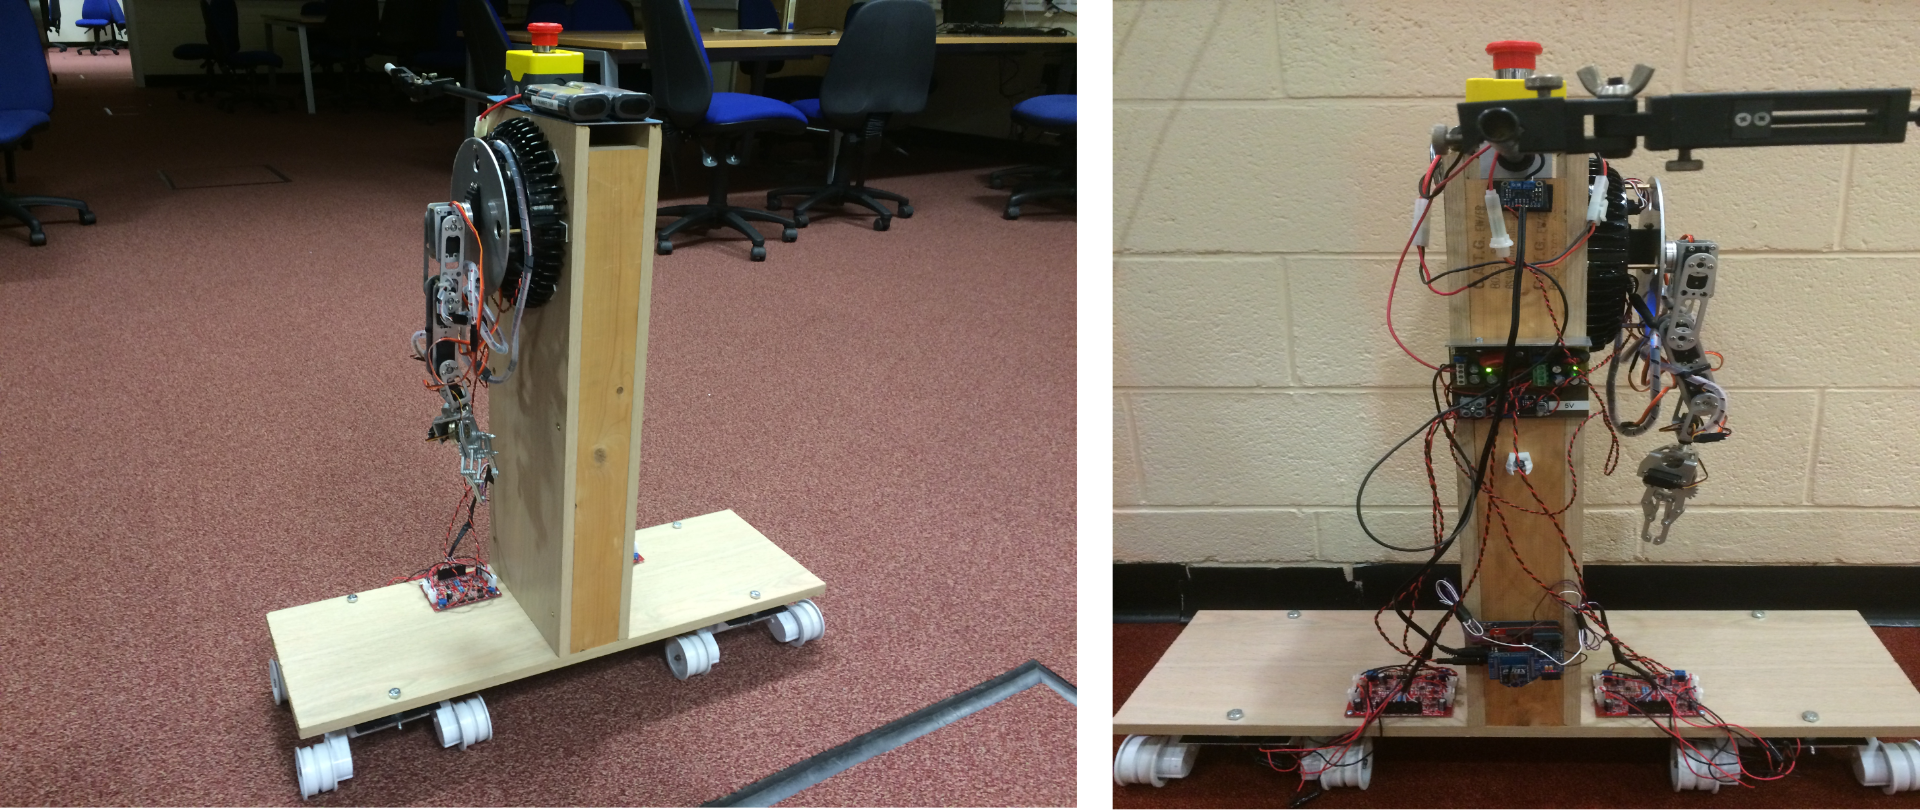
\includegraphics[scale=0.30]{finallook3_low}
\caption{Final Result}
\label{fig:finallook}
\end{center}
\end{figure}

\section{Future Work}
\subsection{Inverse Kinematics}
The current tracking system that operates the robotic arm aims to mimic the user's pose. In numerous scenarios, an \textbf{inverse kinematic} approach would be more viable. Instead of mimicking the configuration of every joint in the arm, the \textbf{IK} approach automatically determines the configuration of all the various joints, by knowing the 3D position of the end-effector, relative to the base of the arm. 
\subsection{Autonomous Capabilities}
The end result of this project has given us a robotic platform that can move and manipulate objects. Autonomous Capabilities could represent a viable step forward, given the existence of a physical platform.


\let\cleardoublepage\clearpage
\begin{appendices}

\chapter{RA1-Pro Schematics}

\begin{figure}[H]
\begin{center}
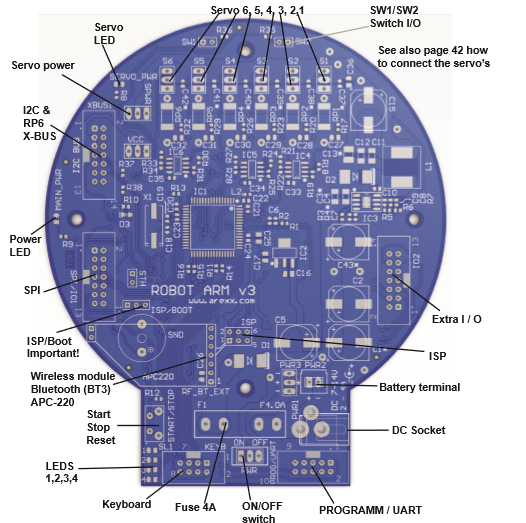
\includegraphics{pcb-arm}
\caption{RA1-Pro PCB, featuring all the various connectors. Note the built in connector for the \textbf{APC-220} wireless module. \cite{arexx}}
\label{fig:pcb-arm}
\end{center}
\end{figure}

\begin{figure}[H]
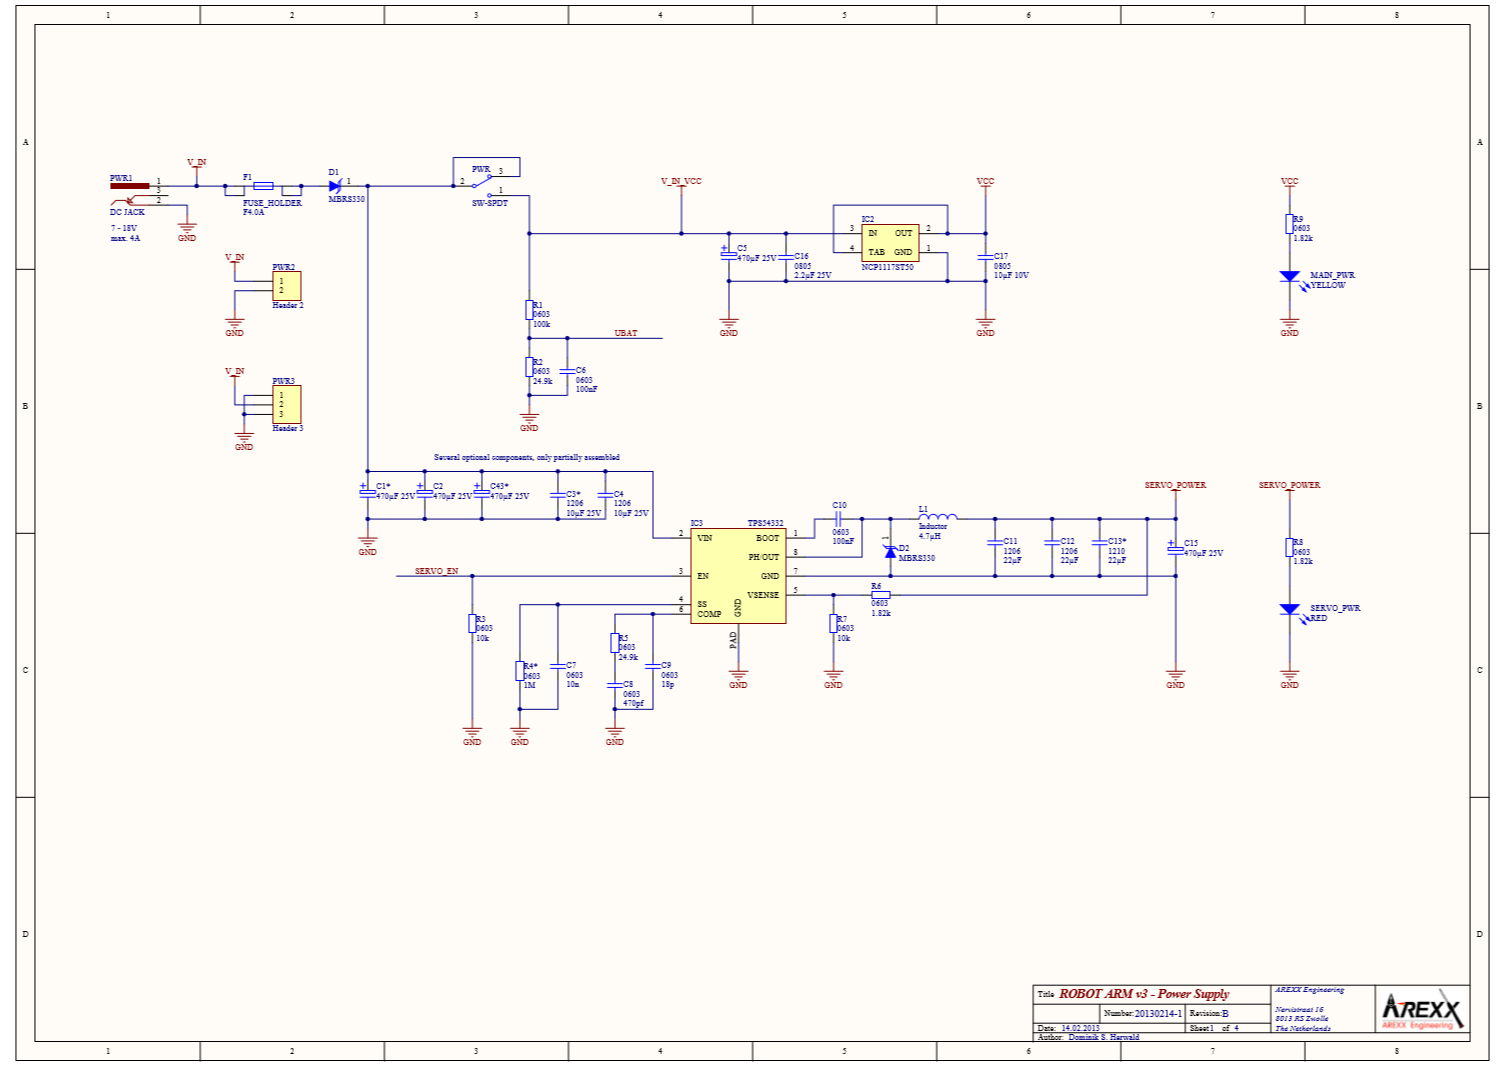
\includegraphics[scale=0.45]{arm-supply-schematic}
\caption{RA1-Pro v3 Power Supply Schematic \cite{arexx}}
\label{fig:arm-supply-schematic}
\end{figure}

\begin{figure}
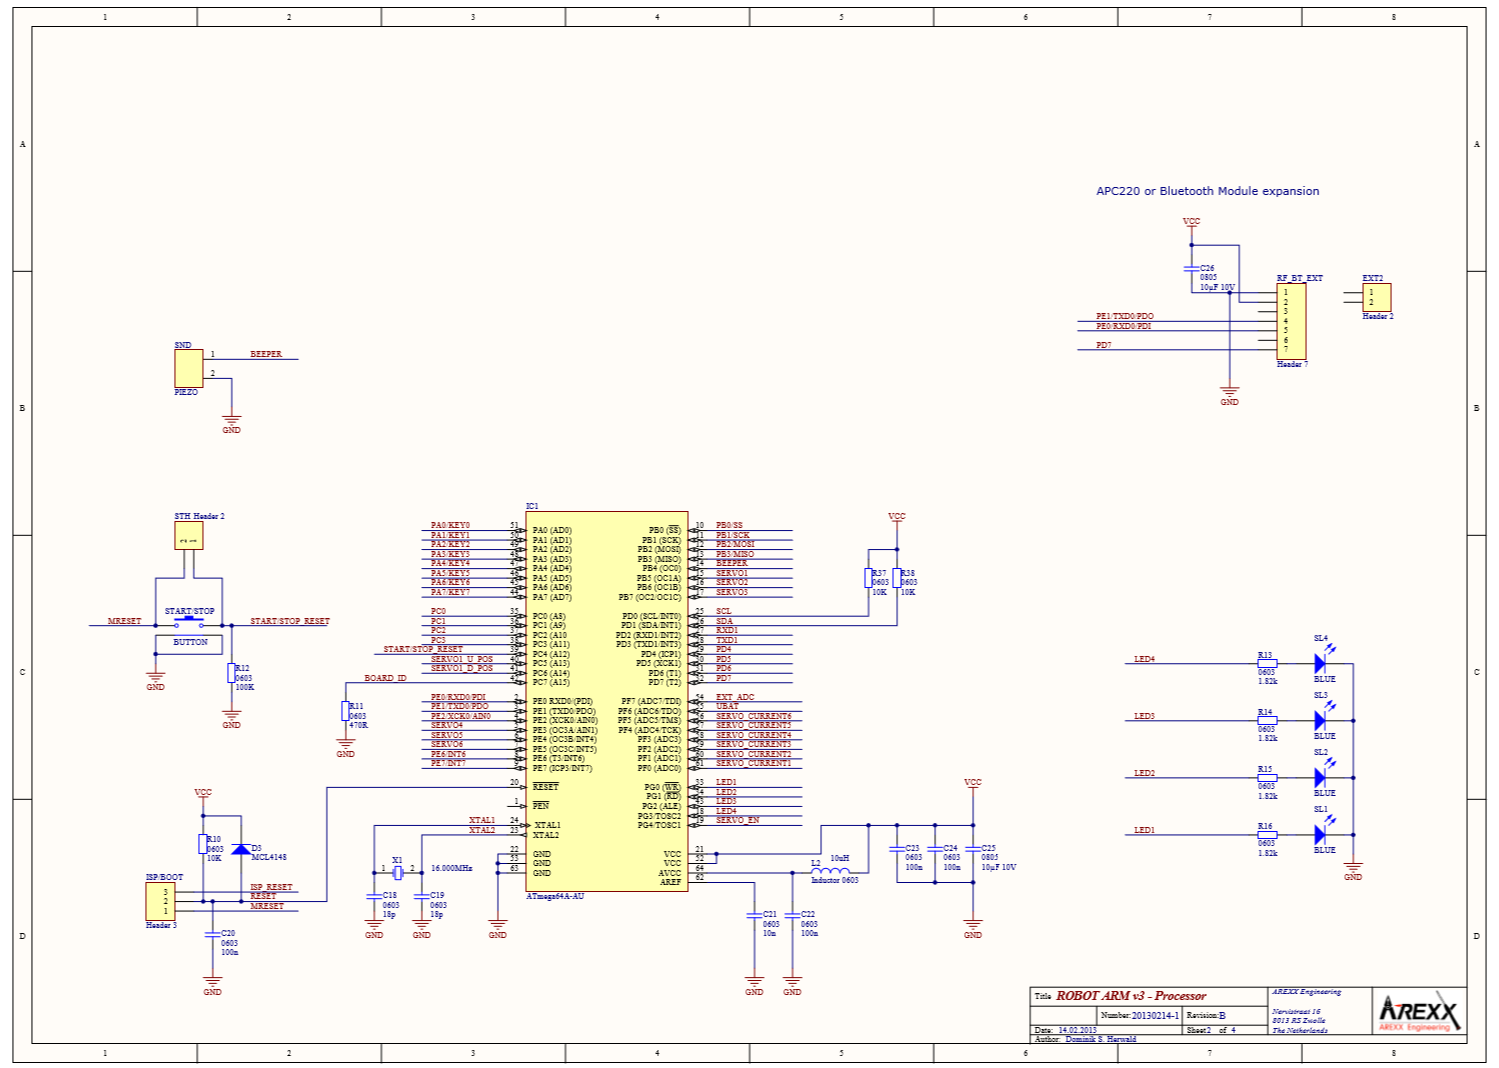
\includegraphics[scale=0.45]{arm-processor-schematic}
\caption{RA1-Pro v3 Processor Schematic \cite{arexx}}
\label{fig:arm-processor-schematic}
\end{figure}
  	
\begin{figure}
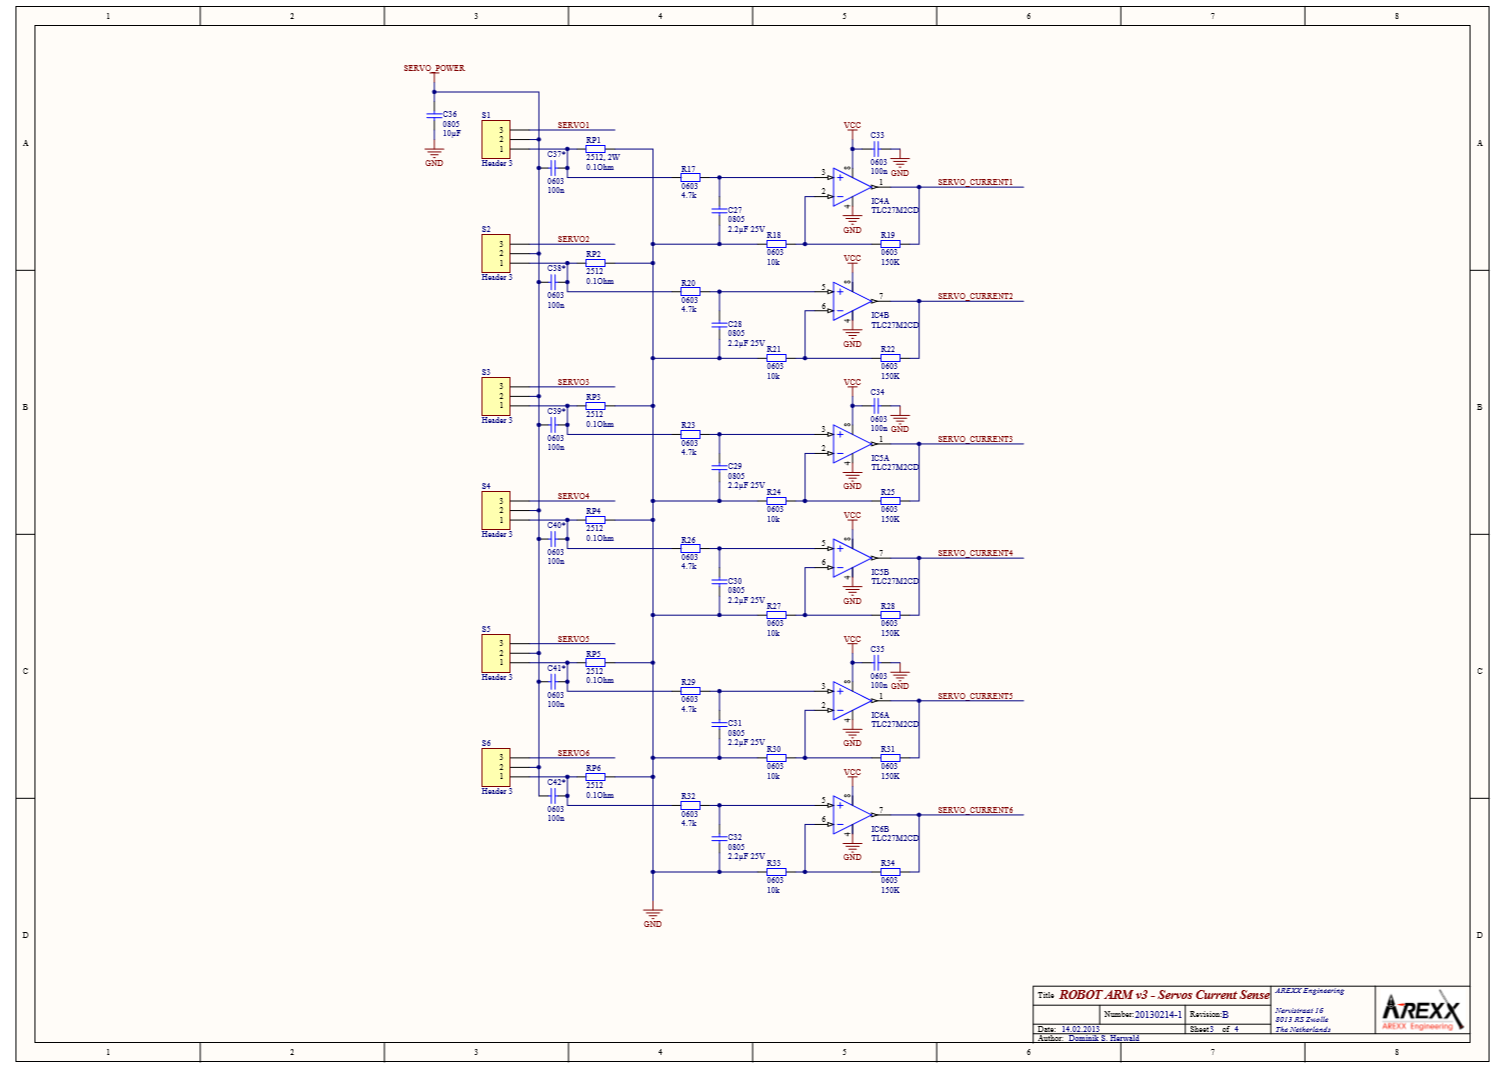
\includegraphics[scale=0.45]{arm-servocurrent-schematic}
\caption{RA1-Pro v3 Servo Current Schematic \cite{arexx}}
\label{fig:arm-supply-schematic}
\end{figure}
  	
\begin{figure}
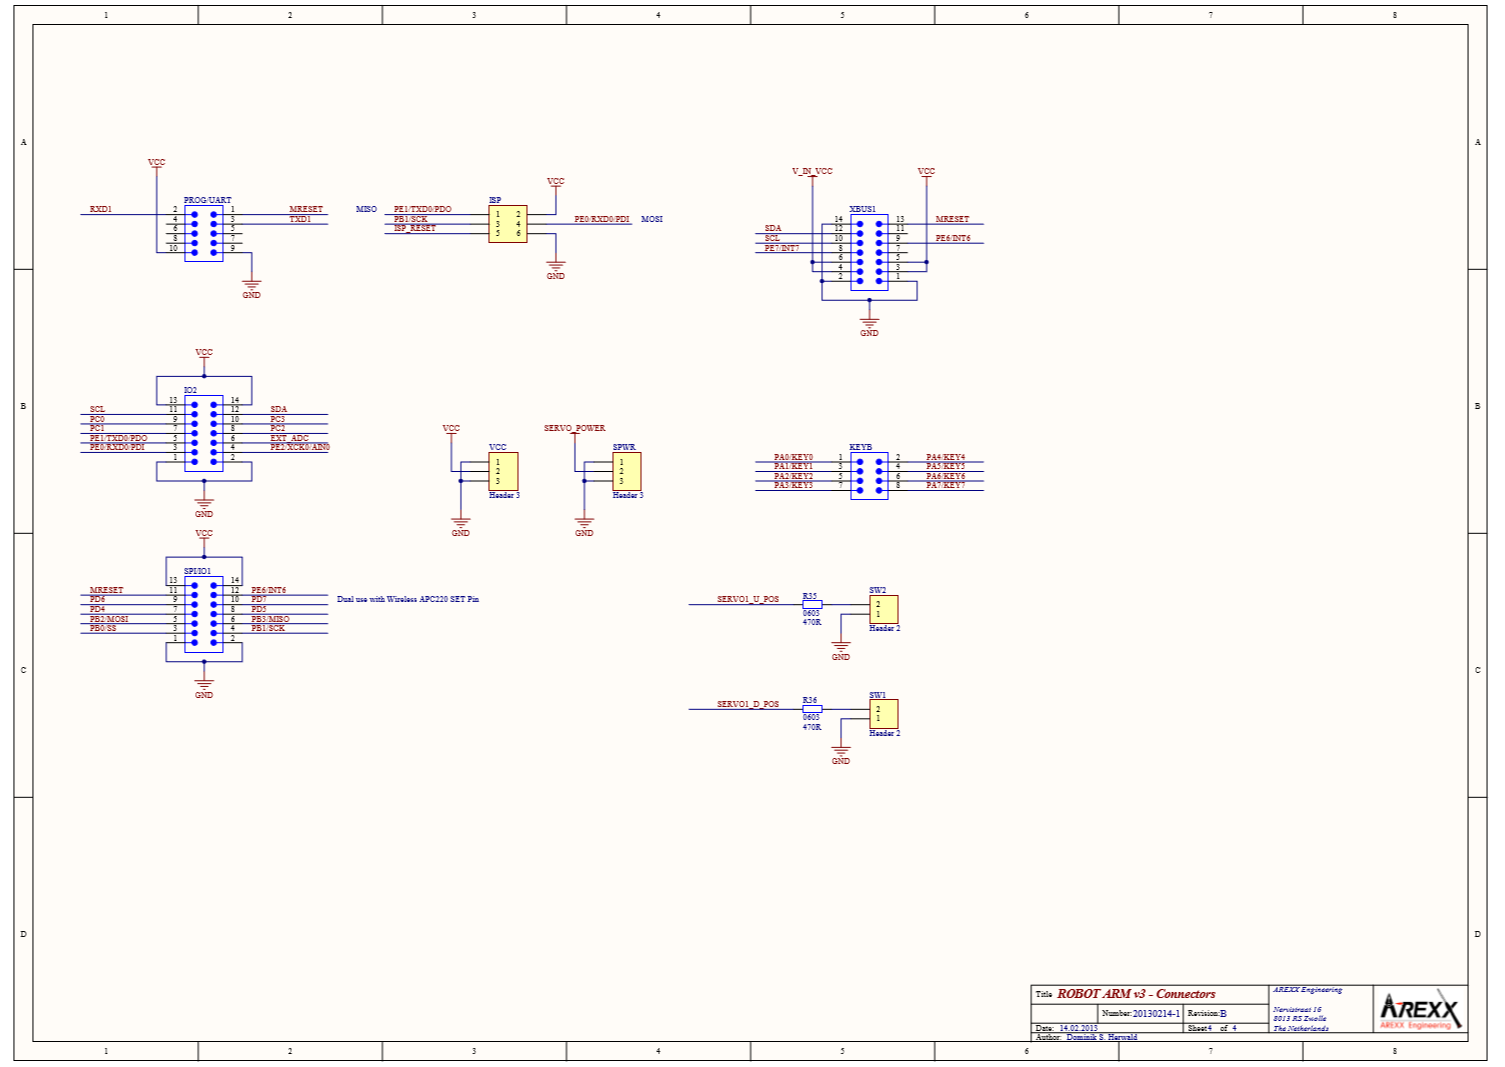
\includegraphics[scale=0.45]{arm-connectors-schematic}
\caption{RA1-Pro v3 Connectors Schematic \cite{arexx}}
\label{fig:arm-connectors-schematic}
\end{figure}
\end{appendices}

\bibliographystyle{unsrt}
\bibliography{mybibliography}


\end{document}
		